\chapter{Experiments}
\label{chap:experiments}

Experiments were conducted in order to validate for the proposed approaches. The goal of these experiments is to determine whether data from an \gls{oss} repository can predict changes that occur within the next 5 commits. These experiments are based on the approach outlined in the previous chapter, \Cref{chap:prediction}. The experiment was conducted through measuring the performance of each core factors varied in isolation. Specifically the \gls{swr}, the feature set and categorization balancing using oversampling. These three factors are explored for both machine learning algorithms.

\section{Experimental Repository Data}
\label{sec:experimental_repository_data}

%One thing that should be noted for the experiments that were run. Since all of the data was known before the model was even created artificial cut off dates were created to allow for the feature set to be tested as to their effect on the model. A test project, acra (developed by the user ACRA), was chosen to develop the method on. 

%The project data was extracted from GitHub from when the project was initially committed to GitHub (2010-04-18 15:52:18-04) till the cut off day of extraction (2015-06-05 09:02:56-04). The cut off day was the day the data was extracted from GitHub and after of which the data analysis was initiated.

The complete list of repositories used in the experiment data are found in \autoref{tab:repositories_summary}. Commit data from each repository was collected from the creation date for the repository till the data collection date. The commit data excludes any commit that lacked a change to a file containing Java code. Since the primary interest was to parse Java code, files containing Java code were used while all other files are ignored. These measures provide a more accurate description of the repository in terms of the analysis and predictions made on it. Secondly, the number of developers does not map effectively to what git uses as committers and authors. Instead, the number of developers includes all individuals (removing duplicates) who committed or authored commits to the current repository.

% TODO consider placing this into introduction
\begin{table}[!hbp]
%\begin{minipage}{\textwidth}
\begin{center}
    \begin{tabular}{|c|c|c|c|c|c|}
        \hline
        \textbf{Owner} & \textbf{Repository} & \textbf{Start Date} & \textbf{End Date} & \textbf{\# of} & \textbf{\# of} \\
         & & & & \textbf{Commits} & \textbf{Developers} \\
        \hline
        ACRA & acra & 2010-04-18 & 2015-06-05 & 404 & 32 \\
        arquillian & arquillian-core & 2009-11-13 & 2016-03-16 & 473 & 49 \\
        google & blockly-android & 2015-07-23 & 2016-06-23 & 691 & 8 \\
        openzipkin & brave & 2013-04-07 & 2016-06-21 & 337 & 32 \\
        gabrielemariotti & cardslib & 2013-09-20 & 2015-05-12 & 327 & 13 \\
        square & dagger & 2012-06-25 & 2016-01-30 & 496 & 38 \\
        deeplearning4j & deeplearning4j & 2013-11-27 & 2016-02-13 & 3523 & 61 \\
        facebook & fresco & 2015-03-26 & 2015-10-30 & 313 & 45 \\
        Netflix & governator & 2012-03-18 & 2016-06-23 & 621 & 31 \\
        greenrobot & greenDAO & 2011-07-28 & 2016-05-23 & 415 & 4 \\
        kevinsawicki & http-request & 2011-10-21 & 2015-01-21 & 273 & 14 \\
        koush & ion & 2013-05-22 & 2016-06-14 & 520 & 29 \\
        skylot & jadx & 2013-03-18 & 2016-03-27 & 480 & 11 \\
        mapstruct & mapstruct & 2012-05-28 & 2016-06-15 & 604 & 22 \\
        Atmosphere & nettosphere & 2012-02-09 & 2016-04-11 & 336 & 12 \\
        johncarl81 & parceler & 2013-07-03 & 2016-06-22 & 228 & 12 \\
        orfjackal & retrolambda & 2013-07-20 & 2016-04-30 & 275 & 11 \\
        amlcurran & ShowcaseView & 2012-08-14 & 2016-05-30 & 332 & 39 \\
        haifengl & smile & 2014-11-20 & 2016-06-24 & 237 & 14 \\
        perwendel & spark & 2011-05-05 & 2016-06-19 & 551 & 86 \\
        apache & storm & 2011-09-16 & 2015-12-28 & 2445 & 260 \\
        prestodb & tempto & 2015-03-06 & 2016-06-20 & 298 & 19 \\
        gridgain & yardstick & 2014-04-11 & 2015-10-12 & 213 & 12 \\
        \hline
    \end{tabular}
\end{center}
\caption{OSS Repositories used in Experiments}
\label{tab:repositories_summary}
%\end{minipage}
\end{table}

\begin{enumerate}
\item \textbf{acra}\footnote{\url{https://github.com/ACRA/acra}} is an Android bug logging tool used with Android applications to capture information related to bugs or crashes. The information is sent to the developers to help them address the issues that their clients encounter while using there application.
\item \textbf{arquillian-core}\footnote{\url{https://github.com/arquillian/arquillian-core}} is a platform for creating automated integration, functional and acceptance tests for Java middleware products. 
\item \textbf{blockly-android}\footnote{\url{https://github.com/google/blockly-android}} provides a native implementation of the blockly library for drag and drop development on Android. 
\item \textbf{brave}\footnote{\url{https://github.com/openzipkin/brave}} provides a Java distributed tracing tool for troubleshooting latency problems and is compatible with Zipkin.
\item \textbf{cardslib}\footnote{\url{https://github.com/gabrielemariotti/cardslib}} is an Android library for creating UI Cards in an Android application.
\item \textbf{dagger}\footnote{\url{https://github.com/square/dagger}} from square is a Java application used to satisfy dependencies for classes to replace the factory model of development.
\item \textbf{deeplearning4j}\footnote{\url{https://github.com/deeplearning4j/deeplearning4j}} is a distributed neural network library that integrates Hadoop and Spark. This application is the largest of the all the repositories and provides a large wealth of data to analyze.
\item \textbf{fresco}\footnote{\url{https://github.com/facebook/fresco}} from facebook is the smallest repository with the shortest development period. This repository provides a library for using images on Android to attempt to solve limited memory issues with mobile devices.
\item \textbf{governator}\footnote{\url{https://github.com/Netflix/governator}} is a library of extensions and utilities that enhances Google's Guice to provide injector life-cycle and object life-cycle.
\item \textbf{greenDAO}\footnote{\url{https://github.com/greenrobot/greenDAO}} provides an Android based light and fast object relational mapping to SQLite database entries.
\item \textbf{http-request}\footnote{\url{https://github.com/kevinsawicki/http-request}} is a library accessing the \textit{httpURLConnection} to make requests and then access the response.
\item \textbf{ion}\footnote{\url{https://github.com/koush/ion}} provides asynchronous networking and image loading for Android.
\item \textbf{jadx}\footnote{\url{https://github.com/skylot/jadx}} is a Java decompiler for Android Dex and Apk files.
\item \textbf{mapstruct}\footnote{\url{https://github.com/mapstruct/mapstruct}} is an annotation processor for generating type-safe bean mapping classes.
\item \textbf{nettosphere}\footnote{\url{https://github.com/Atmosphere/nettosphere}} provides a WebSocket/HTTP server based on Atmosphere and Netty Framework.
\item \textbf{parceler}\footnote{\url{https://github.com/johncarl81/parceler}} is a library for creating serialize code.
\item \textbf{retrolambda}\footnote{\url{https://github.com/orfjackal/retrolambda}} provides a backport for lambda expressions implemented in Java 8 to Java 7, 6 and 5. 
\item \textbf{ShowcaseView}\footnote{\url{https://github.com/amlcurran/ShowcaseView}} is a library for Android that can highlight and showcase components within the UI of a application.
\item \textbf{smile}\footnote{\url{https://github.com/haifengl/smile}} stands for Statistical Machine Intelligence and Learning Engine and is a machine learning library for Java.
\item \textbf{spark}\footnote{\url{https://github.com/perwendel/spark}} a tiny web framework for Java 8.
\item \textbf{storm}\footnote{\url{https://github.com/apache/storm}} from apache real time computational system for continuous streams of data. This repository is one of the larger repositories and has a large development community.
\item \textbf{tempto}\footnote{\url{https://github.com/prestodb/tempto}} A testing framework for SQL databases running on Hadoop.
\item \textbf{yardstick}\footnote{\url{https://github.com/gridgain/yardstick}} is a framework for creating benchmarks specifically for clustered or distributed systems.

\end{enumerate}


Given the large number of repositories, a categorization system was established to group repositories based on similar attributes. Four repository measures were selected for comparing the repositories and are outlined in \autoref{tab:repository_size_summary_info}. The measures are:
\begin{itemize}
\item Repository length in years.
\item Repository size in number of methods.
\item Number of developers.
\item The rate of commits made in commits per year.
\end{itemize}
The repository length represents the number of years the repository has been under development for. The size of the repository is measured in the number of method signatures within the repository since created. The number of developers is tallied from the beginning of the repository for this measure. Finally, the rate of commits is the number of commits contributed to the repository per year. A yearly rate of commits was sufficient since the majority of the repositories had more than one year of development history.

\begin{table}
\begin{center}
    \begin{tabular}{|c|c|c|c|}
        \hline
        \textbf{Repo Duration} & \textbf{Repo Size} & \textbf{\# Devs} & \textbf{Commit Rate} \\
        \hline
        \hline
        short ($t < 1$) & small ($m < 2000$) & small ($d < 30$) & low ($r < 100$) \\
        \hline
        medium & medium & medium & medium \\
        ($1 \leq t < 3$) & ($2000 \leq m < 10000$) & ($30 \leq d < 100$) & ($100 \leq r < 300$) \\
        \hline
        long ($t \geq 3$) & large ($m \geq 10000$) & large ($d \geq 100$) & high ($300 \leq r < 600$) \\
        \hline
        & & & very high ($r \geq 600$) \\
        \hline
    \end{tabular}
\end{center}
\caption{Experiment Repository Summary}
\label{tab:repository_size_summary_info}
\end{table}

% \begin{table}
% \begin{center}
%     \begin{tabular}{|c|c|c|c|c|}
%         \hline
%         project length & short ($t < 12 m$) & medium ($12 m \leq t < 3 y$) & long ($t \geq 3 y$) & \\
%         project size & small ($m < 2000$) & medium ($2000 \leq m < 10000$) & large ($m \geq 10000$) & \\
%         \# devs & small ($d < 30$) & medium ($30 \leq d < 100$) & $d \geq 100$ & \\
%         commit rate & low rate ($r < 100$) & medium ($100 \leq r < 300$) & high rate ($300 \leq r < 600$) & very high rate ($r \geq 600$) \\
%         \hline
%     \end{tabular}
% \end{center}
% \caption{Experiment project summary}
% \label{tab:project_size_summary_info}
% \end{table}

Using the classifications outline in \autoref{tab:repository_size_summary_info}, the repositories are grouped and organized with similar repositories. In \autoref{tab:repository_size_summary} the repositories are sorted by their classification and have dividing lines around similar repositories. For example four repositories; http-request, nettosphere, parceler and retrolambda are all classified in the same group. Some repositories like ion or storm are not grouped in with another repository and thus are in a group of their own.

\begin{table}
\begin{center}
    \begin{tabular}{|c|c|c|c|c|}
        \hline
        \textbf{Repo Name} & \textbf{Repo Duration} & \textbf{Repo Size} & \textbf{\# Devs} & \textbf{Commit Rate} \\
        \hline
        \hline
        yardstick & medium & small & small & medium \\
        \hline
        tempto & medium & medium & small & medium \\
        \hline
        blockly-android & medium & medium & small & high \\
        \hline
        fresco & medium & medium & medium & high \\
        \hline
        http-request & long & small & small & low \\
        nettosphere & long & small & small & low \\
        parceler & long & small & small & low \\
        retrolambda & long & small & small & low \\
        \hline
        ion & long & small & small & medium \\
        \hline
        acra & long & small & medium & low \\
        dagger & long & small & medium & low \\
        ShowcaseView & long & small & medium & low \\
        \hline
        greenDAO & long & medium & small & low \\
        smile & long & medium & small & low \\
        \hline
        cardslib & long & medium & small & medium \\
        jadx & long & medium & small & medium \\        
        mapstruct & long & medium & small & medium \\
        \hline
        arquillian-core & long & medium & medium & low \\
        brave & long & medium & medium & low \\
        spark & long & medium & medium & low \\
        \hline    
        
        governator & long & medium & medium & medium \\
        \hline
        deeplearning4j & long & large & medium & very high \\
        \hline
        storm & long & large & large & high \\
        \hline
    \end{tabular}
\end{center}
\caption{Experiment Repository Summary}
\label{tab:repository_size_summary}
\end{table}

Each of the repositories are selected from GitHub using the list of Java repositories with a large amount of development. \gls{oss} repositories were targeted to simplify any usage concerns. Specifically, \gls{oss} repositories are open and freely available immediately and can be discussed without restriction. Therefore in order to be selected the program had to clearly use an \gls{oss} license. Secondly, the repository also needed to have at least a 6 months worth of development and at least 300 commits to provide a large enough dataset to analyze. An effort was also made to pick repositories of different sizes to provide better tests of various conditions.

\begin{table}
\begin{center}
    \begin{tabular}{|c|c|c|c|c|c|}
        \hline
        \textbf{Repository} & \textbf{\# of} & \textbf{\# of} & \textbf{Avg \# of} & \textbf{Avg \# of} \\
         & \textbf{Methods} & \textbf{Methods} & \textbf{Commits} & \textbf{Methods Change} \\
         & & \textbf{Changes} & \textbf{/ Year} & \textbf{/ Commit} \\
        \hline
        acra & 1309 & 3605 & 67.33 & 9.51 \\
        arquillian-core & 5563 & 6657 & 59.13 & 15.2 \\
        blockly-android & 3608 & 9679 & 345.5 & 14.82 \\
        brave & 4204 & 7823 & 84.25 & 26.98 \\
        cardslib & 3940 & 5122 & 109.0 & 16.68 \\
        dagger & 1827 & 6314 & 99.2 & 13.7 \\
        deeplearning4j & 29896 & 82198 & 880.75 & 24.33 \\
        fresco & 3463 & 4139 & 313.0 & 14.73 \\
        governator & 4229 & 10946 & 124.2 & 19.04 \\
        greenDAO & 4089 & 8625 & 69.17 & 21.84 \\
        http-request & 726 & 1740 & 54.6 & 6.72 \\
        ion & 1678 & 4347 & 130.0 & 8.82 \\
        jadx & 6012 & 9322 & 120.0 & 19.63 \\
        mapstruct & 7885 & 10185 & 120.8 & 19.04 \\
        nettosphere & 1112 & 2857 & 67.2 & 9.01 \\
        parceler & 1619 & 3076 & 57.0 & 14.72 \\
        retrolambda & 1111 & 2588 & 68.75 & 9.95 \\
        ShowcaseView & 927 & 2672 & 66.4 & 8.62 \\
        smile & 3885 & 3879 & 79.0 & 18.47 \\
        spark & 3117 & 9154 & 91.83 & 18.27 \\
        storm & 14599 & 50037 & 489.0 & 24.03 \\
        tempto & 2422 & 3386 & 149.0 & 11.96 \\
        yardstick & 512 & 1216 & 106.5 & 6.37 \\
        \hline
    \end{tabular}
\end{center}
\caption{Repository Change Statistics I}
\label{tab:repository_stats}
\end{table}

In order to get a more detailed understand of the selected repositories, numerous measures were taken. These measures also allow for each repositories to be compared to each other in terms of the development of each of the repositories. For example the size of the repository is represented through several measures including: number of commits, methods and developers. Several averages are calculated to help establish how the development occurred within a repository during the development. A few examples of average measurements are the number of commits per year, changes per method.

\begin{table}
\begin{center}
    \begin{tabular}{|c|c|c|c|c|c|}
        \hline
        \textbf{Repository} & \textbf{Avg \# of} & \textbf{Avg \# of} & \textbf{Avg \# of} & \textbf{Max} & \textbf{Min} \\
         & \textbf{Methods} & \textbf{Changes} & \textbf{Commits /} & \textbf{Commits} & \textbf{Commits} \\
         & \textbf{Change} & \textbf{/ Method} & \textbf{Developer} & \textbf{/ Year} & \textbf{/ Year} \\
         & \textbf{/ Year} & & & & \\
        \hline
        acra & 600.83 & 4.52 & 13.93 & 119 & 33 \\
        arquillian-core & 832.13 & 2.03 & 36.38 & 175 & 6 \\
        blockly-android & 4839.5 & 4.68 & 98.71 & 690 & 1 \\
        brave & 1955.75 & 4.24 & 14.65 & 108 & 56 \\
        cardslib & 1707.33 & 3.28 & 46.71 & 223 & 3 \\
        dagger & 1578.5 & 5.64 & 16.0 & 236 & 4 \\
        deeplearning4j & 20549.5 & 5.69 & 65.24 & 2018 & 65 \\
        fresco & 4139.0 & 1.49 & 156.5 & 313 & 313 \\
        governator & 2189.2 & 4.11 & 24.84 & 159 & 75 \\
        greenDAO & 1437.5 & 3.94 & 138.33 & 137 & 5 \\
        http-request & 348.0 & 2.56 & 39.0 & 108 & 5 \\
        ion & 1086.75 & 3.31 & 40.0 & 253 & 7 \\
        jadx & 2330.5 & 2.41 & 43.64 & 208 & 11 \\
        mapstruct & 2037.0 & 2.04 & 54.91 & 288 & 7 \\
        nettosphere & 571.4 & 4.37 & 37.33 & 118 & 5 \\
        parceler & 769.0 & 2.43 & 45.6 & 76 & 41 \\
        retrolambda & 647.0 & 3.06 & 25.0 & 133 & 24 \\
        ShowcaseView & 534.4 & 5.9 & 10.71 & 141 & 6 \\
        smile & 1293.0 & 1.86 & 19.75 & 121 & 6 \\
        spark & 1525.67 & 3.92 & 7.25 & 171 & 22 \\
        storm & 10007.4 & 5.93 & 15.47 & 948 & 118 \\
        tempto & 1693.0 & 1.88 & 16.56 & 253 & 45 \\
        yardstick & 608.0 & 3.65 & 23.67 & 208 & 5 \\
        \hline
    \end{tabular}
\end{center}
\caption{Repository Change Statistics II}
\label{tab:repository_stats_2}
\end{table}

% TODO reference the table
Several average measures were also taken which detail the amount of change that occurs within the repository. The average number of commits per repository coupled with the average number of changes per commit clearly indicates the amount of changes that are occurring with in the repository. The rate at which methods are change provides good insight into the growth of a repository. While some changes may involve the addition of new methods, others may include the removal of methods or the modification of methods. The other measures relating to the amount of change occurring with a repository on average are the number of methods changed per year and the number of changes per method. Each of these further outline how the changes are being made to the repository on average.

A few of the measures are related to the number of developers. These while provided are not the primary focus. The information provided by tracking developer interactions with each other or the repository could be integrated into future work.

\begin{table}
\begin{center}
    \begin{tabular}{|c|c|c|c|c|c|}
        \hline
        \textbf{Repository} & \textbf{Max \# of} & \textbf{Min \# of} & \textbf{Max \# of} & \textbf{Max \# of} & \textbf{Min \# of} \\
         & \textbf{Methods} & \textbf{Methods} & \textbf{Change /} & \textbf{Commits /} & \textbf{Commits /} \\
         & \textbf{Changed} & \textbf{Changed} & \textbf{Method} & \textbf{Developer} & \textbf{Developer} \\
         & \textbf{/ Year} & \textbf{/ Year} & & & \\
        \hline
        acra & 1503 & 183 & 52 & 229 & 1 \\
        arquillian-core & 3421 & 55 & 110 & 420 & 1 \\
        blockly-android & 9543 & 136 & 90 & 538 & 1 \\
        brave & 3300 & 1038 & 83 & 225 & 1 \\
        cardslib & 3340 & 19 & 95 & 285 & 1 \\
        dagger & 3374 & 171 & 65 & 157 & 1 \\
        deeplearning4j & 35869 & 4377 & 345 & 1987 & 1 \\
        fresco & 4139 & 4139 & 33 & 269 & 44 \\
        governator & 3324 & 1066 & 263 & 316 & 1 \\
        greenDAO & 2971 & 34 & 63 & 367 & 1 \\
        http-request & 752 & 14 & 50 & 267 & 1 \\
        ion & 2315 & 24 & 161 & 492 & 1 \\
        jadx & 3915 & 248 & 197 & 436 & 1 \\
        mapstruct & 4462 & 201 & 81 & 334 & 1 \\
        nettosphere & 1074 & 10 & 46 & 322 & 1 \\
        parceler & 1151 & 516 & 31 & 217 & 1 \\
        retrolambda & 1501 & 212 & 83 & 237 & 1 \\
        ShowcaseView & 1156 & 74 & 70 & 215 & 1 \\
        smile & 1918 & 872 & 24 & 155 & 1 \\
        spark & 2818 & 277 & 72 & 277 & 1 \\
        storm & 26526 & 2152 & 314 & 622 & 1 \\
        tempto & 3073 & 313 & 44 & 66 & 1 \\
        yardstick & 1163 & 53 & 62 & 137 & 1 \\
        \hline
    \end{tabular}
\end{center}
\caption{Repository Change Statistics III}
\label{tab:repository_stats_3}
\end{table}

While the purposed method was being developed ACRA's acra repository was primarily used for exploring and initial testing of the approach. After experimenting on acra a few of the potential candidate feature sets were distinguished based on their superior performance. Experiments were then run on other repositories using the feature sets that performed better.

\section{Experimental Setup}


The experimental setup defines numerous parameters of different importance to conduct experiments. The majority of these parameters will remain constant to help observe the impact differences in the independent variable will have on the three dependent variables; precision, recall and accuracy. Each experiments will use one of the parameters as the independent variable. The three independent variables used in the experiments are outlined below. An experiment consists of a set of trails where the independent variable is modified to measure the resulting dependent variables. The results of a single trial or of the set of trails for a repository will be referred to as the performance of the approach. In order to reduce specific repository confounding factors numerous repositories were tested on. This will be discussed further in the discussions section. The experiments section only includes a small sample of the repositories that were experimented on. The repositories shown are ones that exhibited interesting patterns or results. The complete set of performance figures for every repository are shown in \autoref{app:experimental_data}.

This thesis works to determine whether \gls{svm} or \gls{rf} can be used to effectively predict changes that will occur within the repository. To potentially provide an answer to this question the factors that are used for the prediction method are studied. The experiments attempt to determine what impact the different factors will have on the purposed methods. These factors include:
\begin{enumerate}
\item The \gls{swr} which is the size of range which the samples are taken from.
\item The set of features used to train the machine learning model.
\item The distribution of the data through use of oversampling.
\end{enumerate}

Through investigating these factors a more clear picture of the performance of the approach will be be provided. Without such a investigation the method contains could produce capable solution just as likely as poor solutions. Worse still, the setup may produce poor solutions more often than capable solutions. Once a more concrete understanding is developed of the different factors and the performance of the algorithm accordingly the research question can be answered as to whether it is possible to predict changes within a repository using the commit data.

\subsection{Prediction Features}

%The experimental process for testing the various feature sets on acra involved dividing the repository into four equal quarters (based on time duration). While the number of commits within each period may vary greatly, only a sample is taken.

    %- Alternatively the periods could be distributed such to make the number of commits equal between the sections. Further testing is needed to determine which method is more ideal.

%The \gls{svm} model was trained to categorize whether the current method would be changed within the next 5 commits. This of course can generalize to whether a vector will have a commit within the next \textit{n} commits. Obviously each candidate feature leverages historical or current information and thus a vector can be generated without future information.


%TODO write algorithm for mapping names

% TODO discuss sampling range methods



%An issue that was necessary to address was the arbitrary sample size. For projects that are a lot bigger 100 vectors which map to 100 method changes could be very small. The sampling also seemed like a peculiar approach to picking the data since it would randomly pick values from over a period that could vary from a few months to a few years depending on the size. Therefore instead of dividing the project into four quarters based on time a number of commits is picked. 

% TODO provide an actual start to this subsection
The experimental design to allow for the predictions made on historical data to be tested with available data. Therefore within the data collected for the repository the predictions must be made for values that are already known to allow for verification. Therefore the experimental sampling would build off of the prediction sampling outlined in \Cref{sec:prediction_data}. A second region defined as the prediction sample range. The \autoref{fig:data_range} outlines the updated layout. The size of the training range ($|s_t|$) and the size of the prediction ($|s_p|$) are able to be different sizes, however for each experiment they remain the same ($|s_t| = |s_p|$).

%The population is sampled by percentage of the total available. This allows more flexibility and determining the sample size of a test by allowing for it to scale based on the size of the project. 

% TODO show a final picture with population size as a percentage.

% TODO access this stuff below. Remember It's now 5 commits not 6 and also a lot of this stuff is no longer relevant.

%The initial thought was to provide a few different features that appeared to be unique and potentially provided useful information for whether the method will change within the next 5 commits. Of course since this measurement is calculated, if a vector within the sample set is within the last 5 commits then it will leverage data from the next quarter to provide its prediction. This has not been mitigated and could provide a unrealistic improvement in the prediction score if members of the next sample fall into the first 5 commits. The way to mitigate this would be to provide a buffer between the two sets when the second test is used for testing purposes. The second set would be restricted further, such that the changes must come from after the 6th commit from the start date of the quarter. The first commit would be the one that takes place on or right after (if no commit falls on that date) the start date. The next 5 commits would also be excluded from the test sample set.

%\subsection{Experiment Factors}
% TODO outline the different factors used in the experiments. Also even outline other factors that are not changed either.

% Factors:
% Sliding Window
% Extended sampling ranges
% Training Range
% Testing Range
% Sample Range by Commit (or by date)
% Oversampling
% Undersampling
% Dynamic Size of sampling
% Sampling Percent
% Sampling Randomly
% Window
% SVM or Forest Parameters

The sample range is taken from the current commit $c_i$ to $c_{i-g-m}$ in the case that $i > m$. $m$ denotes the size of \gls{swr} in commits and $g$ is the number of commits the change is predicted within. For example if the model is predict a change that occurs within the next 5 commits ($g = 5$) and $m = 30$ then \autoref{fig:data_range} shows how the data would be sampled. The training sample would be where data would be collected from to train the model. The prediction gap is to account for the data sampling calculating whether methods at commit 40 will have a change within the next 5 commits. Therefore to properly test it on data that is not used as part of the testing model the offset is needed. The \gls{swr} for the testing data set is labeled as the \textit{Testing Sampling}.

% TODO include a table/list about each of the features (similar to tab:candidate_features)

The sliding window factor is one of core aspects related to extracting samples from the data set. When using the sliding window to sample the data the data is divided as shown in \autoref{fig:data_range}. The training sample is where the training data set is sampled from. The testing sample is where the testing data is sampled from. 

\begin{figure}[!ht]
    \centering
        %Generated from http://jsfiddle.net/toufm01e/
        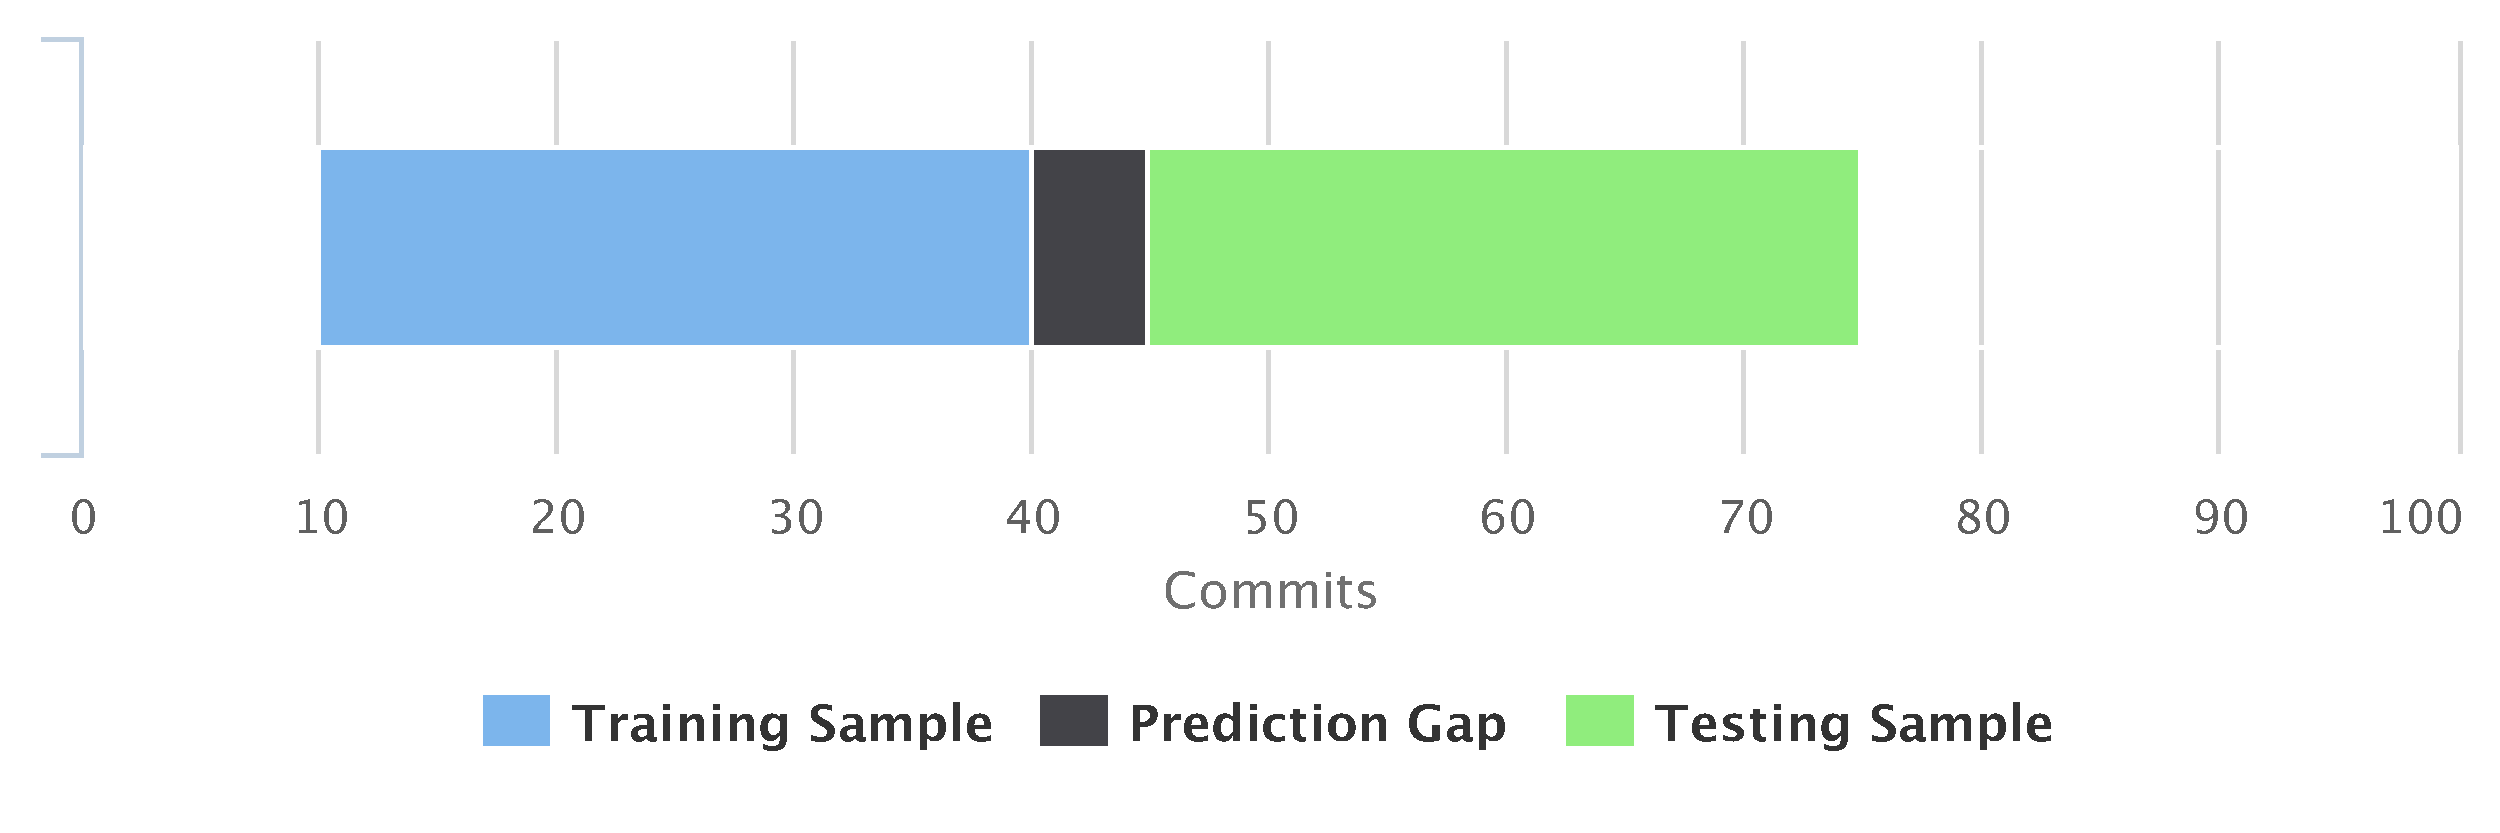
\includegraphics[width=1.0\textwidth]{images/exp_data_range}
    \caption{Sampling Window Layout}
    \label{fig:data_range}
\end{figure}


A data set with an extended sampling range will extend the sampling range beyond the original size for either the training sample or the testing sample. The training range can be expanded to include earlier samples to increase the sample space.

The training and testing sampling range are defined as the number of commits from which the samples can be taken. In \autoref{fig:data_range}, both the training and testing sample ranges are set to 30 commits. These two values can differ from one another but tend to be kept the same for most of the experiments.

As discussed in \Cref{sec:prediction_data}, sample biasing can cause the distribution to favor the selection of one category over another. Undersampling and oversampling can prevent the model from simply classifying all samples as one category or the other.

For each repository data set there are numerous windows that be can be used. The window number is setting which window is used broadly mapping to the position within the data set that the model will be trained on and then predicted on. In \autoref{fig:data_range} the \textit{current commit} is located at 45. This is the point from which predictions will be made after. The gap preceding the starting point is is 5 commits long and is followed by the sample window for the training data which is 30 commits long. To calculate the window offset simply using the starting position ($p_s$), the gap length ($g$), and the \gls{swr} can be calculated in \autoref{eq:window_offset}. Therefore in this case the window offset would be $45 - 5 - 30$ which is 10.

\begin{equation} 
\label{eq:window_offset}
wo = p_s - g - swr 
\end{equation}

Finally, the last factor of note is the parameters used to configure each prediction method. \gls{rf} use a single parameter, the size of the forest. \gls{svm} meanwhile uses two parameters; C and gamma. Picking the most suitable parameters is ideal to achieve good performance from the prediction model. For \gls{svm} a grid search technique is provided by the developers of the libsvm source\footnote{\url{https://www.csie.ntu.edu.tw/~cjlin/libsvm/}} for optimizing the parameters. For \gls{rf}, the size of the forest will have an impact but is far more manageable since it is a single parameter. A larger number of trees in the forest will generally provide better results, but will cause the algorithm to take longer to train.

\subsection{Prediction Performance}

% TODO this isn't necessary for cases when the entire sample is used.
For each experiment where the used random sampling the experiment was performed 5 times to account for variations in the random sample. Therefore if the initial results using the first sample set were not characteristic of the full dataset then running the experiment with more random samples is more likely to represent the true characteristics of the dataset. This required taking five random samples from each quarter, training the model and running the tests on the model to then determine the average prediction score. %In the case when $100\%$ of the sample is used then only one sample is is taken since there will be no variations within the sample set.

The goal of the prediction methods are to provide a good prediction of whether the a given vector will fit in one category or the other. A model's prediction performance can be rated using three measures of accuracy, precision and recall. Accuracy is measured as how often predictions $p_i$ are classified correctly where $a_i$ represents vector $v_i$ correct classification. The prediction accuracy ($P_{accuracy}$) can then be calculated using \autoref{eq:prediction_accuracy}. This simply sums up the accuracy for each vector and then divides it by the total number of vectors (where $n = |v|$).

% TODO integrate these
\begin{equation}
\label{eq:true_positive}
tp = \sum_{i=0}^{n}\left\{\begin{matrix}
1 & \text{if } p_i = a_i \text{ \& } a_i = 1\\ 
0 & \text{otherwise}
\end{matrix}\right.
\end{equation}

\begin{equation} 
\label{eq:true_negative}
tn = \sum_{i=0}^{n}\left\{\begin{matrix}
1 & \text{if } p_i = a_i \text{ \& } a_i = 0\\ 
0 & \text{otherwise}
\end{matrix}\right.
\end{equation}

\begin{equation}
\label{eq:false_positive}
fp = \sum_{i=0}^{n}\left\{\begin{matrix}
1 & \text{if } p_i \neq a_i \text{ \& } a_i = 0\\ 
0 & \text{otherwise}
\end{matrix}\right.
\end{equation}

\begin{equation}
\label{eq:false_negative}
fn = \sum_{i=0}^{n}\left\{\begin{matrix}
1 & \text{if } p_i \neq a_i \text{ \& } a_i = 1\\ 
0 & \text{otherwise}
\end{matrix}\right.
\end{equation}

\begin{equation}
\label{eq:prediction_accuracy}
P_{accuracy} = \frac{tp+tn}{tp+tn+fp+fn} \times 100
\end{equation}

The precision of a model is the measure of how correct the model predicts that a change will occur when it predicts that a change will occur. Given the true positives $tp$, represents the number of predictions that the model correctly identified as having a change and the false positives $fp$ is the number of times the model incorrect predicted a change to occur when it in fact did not. The equation for calculating precision is show in \autoref{eq:precision}.



\begin{equation} 
\label{eq:precision}
P_{precision} = \frac{tp}{tp+fp}
\end{equation}

The recall of the model is the measure of how correct the model predicts that change will occur out of all the times changes really occurred. Again using $tp$ as the number of true positives, and false negatives $fn$ which is the number of times the model fails to predict that a change will occur. The recall can be calculated using the \autoref{eq:recall}.

\begin{equation} 
\label{eq:recall}
P_{recall} = \frac{tp}{tp+fn}
\end{equation}

\section{Experimental Results}
\label{sec:experimental_results}

% TODO give a brief introduction to experiments. Reference the data discussed in previous sections in this chapter.
% TODO reference the appendix which contains a complete set of figures related to the experiments conducted.

For each experiment all of the data used to train and test the model is collected using a Ruby script to query a PostgreSQL database. The PostgreSQL database provides the raw data which is then processed into data vectors in an acceptable form for \gls{svm} or \gls{rf}. The data processing method is outlined more completely in \Cref{sec:prediction_method}.

\subsection{SVM Experiments}
\label{subsec:svm_experiments}

For this set of experiments the machine learning algorithm \gls{svm} is used to provide the change predictions. As noted in \Cref{sec:prediction_method}, the implementation for \gls{svm} is a Ruby binding of the original library. The parameters used for all of the experiments with \gls{svm} are $C = 10$ and $gamma = 8$.


\subsubsection{Window Range Experiments}
\label{sec:svm_swr_experiment}


In this experiment the independent variable is the size of the \gls{swr} in commits. For each variation of the \gls{swr} the performance is measured. In \autoref{tab:svm_window_range_experiment_features}, the features used by the prediction model are outlined. Features with a mark, $\bullet$, are used while those without are not. In this experiment only the $sf_{\Delta}$ is not used while all the rest are. Each of these features is outlined in further detail in \autoref{tab:candidate_features}.

\begin{table}[h]
\begin{center}

    \begin{tabular}{|c|c|c|c|c|c|c|c|}
        \hline
        Com & Sig & Name & $f_{\Delta}$ & $sf_{\Delta}$ & $t_\Delta$ & Length & $change_{t-1}$ \\
         %& & & & & & & \\
        \hline
        $\bullet$ & $\bullet$ & $\bullet$ & $\bullet$ & & $\bullet$ & $\bullet$ & $\bullet$ \\ \hline
    \end{tabular}
    \caption{\gls{swr} Experiment Features}
    \label{tab:svm_window_range_experiment_features}
\end{center}
\end{table}

As noted above the independent variable for this experiment is the \gls{swr}. The remaining parameters for the experiment are constant for each test. These parameters for this experiment are outlined in \autoref{tab:svm_window_range_experiment_setup}.

\begin{table}[h]
\begin{center}

    \begin{tabular}{|c|c|c|c|c|cc|}
        \hline
        \textbf{Extended} & \textbf{Over} & \textbf{Under} & \textbf{Sample} & \textbf{Window} & \textbf{SVM} & \\
        \textbf{Window} & \textbf{Sampling} & \textbf{Sampling} & \textbf{Rate} & \textbf{Offset} & \textbf{C} & \textbf{gamma} \\ \hline
        No & No & Yes & $100\%$ & 5 & 10 & 8 \\ \hline
    \end{tabular}
    \caption{\gls{swr} Experiment Setup}
    \label{tab:svm_window_range_experiment_setup}
\end{center}

\end{table}

Each repository was tested on using these outlined parameters for an \gls{swr} varying from 60 to 130 by intervals of 10. The results for the experiments are shown with the precision, recall and accuracy. For each graph the independent variable is the number of commits in the \gls{swr}. Y-axis is the percentage for either the precision, recall or accuracy. The complete set of experimental performance results are found in \autoref{app_sub:experiment_1_svm}. For some repositories did not have enough data to complete the entirety of this experiment. For example, smile did not have enough data to complete the trials with \gls{swr} for 120 or 130. These repositories were still included and show how the method works with smaller amount of data available.

% List of projects for this section:
% tempto *pre-groups 1
% http-request *group 2
% acra *group 3
% smile *group 4-5
% spark * group 6+

% TODO rework the following to be the key figures.

The majority of the repositories using \gls{svm} did not perform well with accuracy and precision typically between $0.4$ and $0.6$. This repositories as well as others have very poor results and show the difficulty of this problem. Similarly, \autoref{fig:test_1_blockly-android_svm-exp} shows low precision and accuracy while very high recall. The independent variable, \gls{swr} has very little impact on the performance for this repositories in particular.


\begin{figure}[!ht]
    \centering

        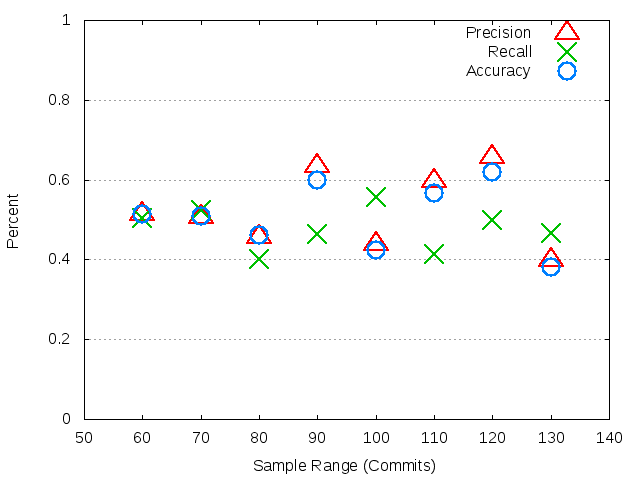
\includegraphics[width=0.8\textwidth]{images/svm/test_1/tempto_sample_range}
        \caption{\gls{swr} for tempto using \gls{svm}}
        \label{fig:test_1_tempto_svm-exp}
\end{figure}

\begin{figure}[!ht]
    \centering

        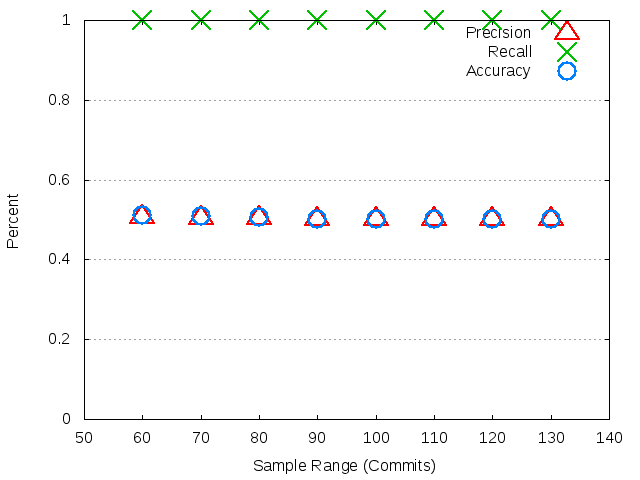
\includegraphics[width=0.8\textwidth]{images/svm/test_1/blockly-android_sample_range}
        \caption{\gls{swr} for blockly-android using \gls{svm}}
        \label{fig:test_1_blockly-android_svm-exp}
\end{figure}

Some of the repositories like http-request in \autoref{fig:test_1_http-request_svm-exp} had a large amount of variation with the changes to the \gls{swr}. In one case http-request moderately well in \gls{swr} 80 while at 60 and 120 the accuracy and recall are $0$.

\begin{figure}[!ht]
    \centering

        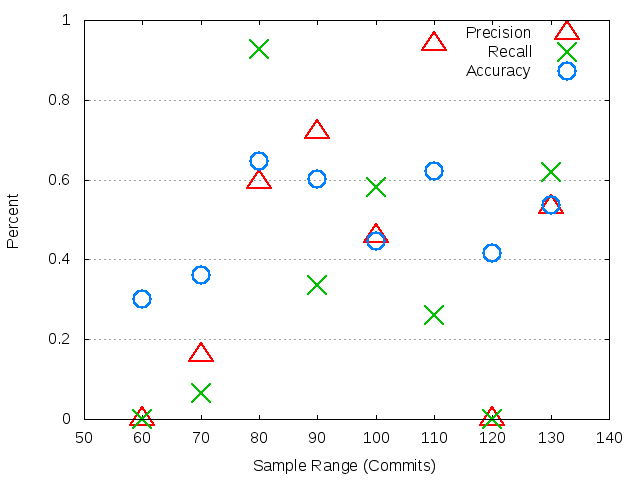
\includegraphics[width=0.8\textwidth]{images/svm/test_1/http-request_sample_range}
        \caption{\gls{swr} for http-request using \gls{svm}}
        \label{fig:test_1_http-request_svm-exp}
\end{figure}

In \autoref{fig:test_1_acra_svm-exp}, the repositories acra is shown with the best result for \gls{svm}. When the \gls{swr} is at 70-100 the performance is high, for the other cases the performance is lower but not by a large margin. The point of interest is that recall performs well for an \gls{swr} of 100 or lower but performs worse than the accuracy and precision after 100.

\begin{figure}[!ht]
    \centering

        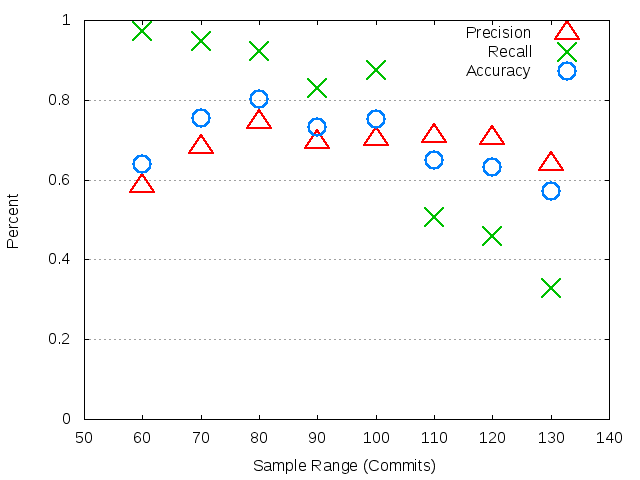
\includegraphics[width=0.8\textwidth]{images/svm/test_1/acra_sample_range}
        \caption{\gls{swr} for acra using \gls{svm}}
        \label{fig:test_1_acra_svm-exp}
\end{figure}

\begin{figure}[!ht]
    \centering

        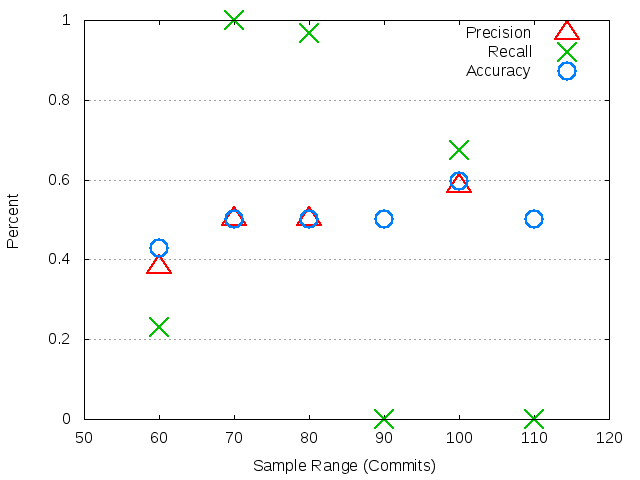
\includegraphics[width=0.8\textwidth]{images/svm/test_1/smile_sample_range}
        \caption{\gls{swr} for smile using \gls{svm}}
        \label{fig:test_1_smile_svm-exp}
\end{figure}

\begin{figure}[!ht]
    \centering

        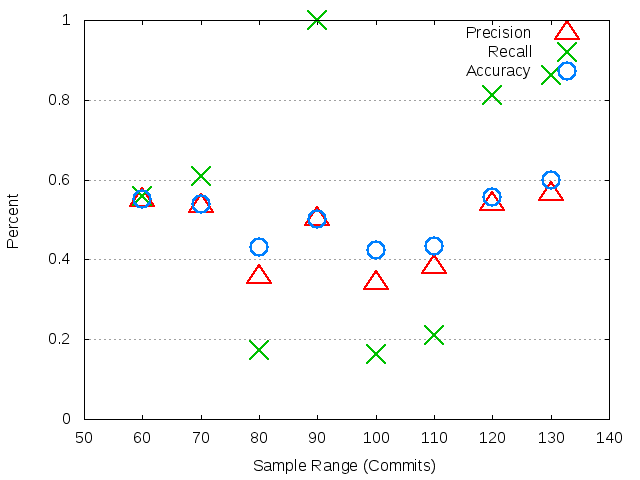
\includegraphics[width=0.8\textwidth]{images/svm/test_1/spark_sample_range}
        \caption{\gls{swr} for spark using \gls{svm}}
        \label{fig:test_1_spark_svm-exp}
\end{figure}

Both smile in \autoref{fig:test_1_smile_svm-exp} and spark in \autoref{fig:test_1_spark_svm-exp} performed poorly each with performance measure below $0.5$. In two cases (90 and 110) smile and 0 recall and undefined precision.

\begin{table}
\begin{center}
    \begin{tabular}{|c||c|c||c|c|c|}
        \hline
        \textbf{Repository} & \textbf{AI} & \textbf{SWR} & \textbf{Precision} & \textbf{Recall} & \textbf{Accuracy} \\
        \hline
        acra & SVM & 100 & 0.74 & 0.92 & 0.8 \\
        arquillian-core & SVM & 70 & 0.55 & 0.71 & 0.57 \\
        blockly-android & SVM & 60 & 0.51 & 1.0 & 0.51 \\
        brave & SVM & 90 & 0.52 & 0.58 & 0.52 \\
        cardslib & SVM & 90 & 0.58 & 0.5 & 0.57 \\
        dagger & SVM & 60 & 0.65 & 0.68 & 0.66 \\
        deeplearning4j & SVM & 120 & 0.58 & 0.55 & 0.58 \\
        fresco & SVM & 130 & 0.57 & 0.67 & 0.58 \\
        governator & SVM & 110 & 0.62 & 0.5 & 0.6 \\
        greenDAO & SVM & 60 & 0.5 & 1.0 & 0.5 \\
        http-request & SVM & 80 & 0.59 & 0.93 & 0.65 \\
        ion & SVM & 70 & 0.56 & 0.62 & 0.57 \\
        jadx & SVM & 130 & 0.55 & 0.82 & 0.58 \\
        mapstruct & SVM & 70 & 0.6 & 0.88 & 0.65 \\
        nettosphere & SVM & 100 & 0.57 & 0.64 & 0.58 \\
        parceler & SVM & 70 & 0.66 & 0.54 & 0.63 \\
        retrolambda & SVM & 80 & 0.52 & 0.96 & 0.53 \\
        ShowcaseView & SVM & 120 & 0.59 & 0.85 & 0.63 \\
        smile & SVM & 100 & 0.58 & 0.67 & 0.6 \\
        spark & SVM & 130 & 0.56 & 0.86 & 0.6 \\
        storm & SVM & 100 & 0.51 & 0.7 & 0.52 \\
        tempto & SVM & 120 & 0.66 & 0.5 & 0.62 \\
        yardstick & SVM & 70 & 0.55 & 0.79 & 0.57 \\
        \hline
    \end{tabular}
\end{center}
\caption{\gls{swr} Repository Best Performance using \gls{svm}}
\label{tab:svm_swr_repository_performance}
\end{table}

The best results for each repositories are outlined in \autoref{tab:svm_swr_repository_performance}. Overall there was no clear value for the \gls{swr} which held consistent positive results. Repositories from similar groups tended to perform similarly. For example acra, dagger and ShowcaseView all tended to perform well for similar parameters. 

Repositories that were influenced more by \gls{swr} thus having a larger variation between values proved to have better results more often however this was not guaranteed. No value of \gls{swr} works across repositories and even for repositories that worked the correct value had to be found in order to obtain good results.
    
\subsubsection{Feature Set Experiments}
\label{sec:svm_feature_set_experiments}


\begin{table}[h]
\begin{center}

    \begin{tabular}{|c|c|c|c|c|c|cc|}
        \hline
        \textbf{Extended} & \textbf{Over} & \textbf{Under} & \textbf{Sample} & \textbf{Window} & \textbf{SWR} & \textbf{SVM} & \\
        \textbf{Window} & \textbf{Sampling} & \textbf{Sampling} & \textbf{Rate} & \textbf{Offset} &  & \textbf{C} & \textbf{gamma} \\ \hline
        No & No & Yes & $100\%$ & 5 & 90 & 10 & 8 \\ \hline
    \end{tabular}
    \caption{Feature Experiment Setup}
    \label{tab:svm_feature_experiment_setup}
\end{center}

\end{table}

% Extend Window: No% Sample by Commit Range: Yes
% Over Sampling: No
% Under Sampling: Yes
% Sample Rate: 100%
% Window Offset: 5
% SVM c: 10
% SVM gamma: 8
% SVM esp: 0.001

%The parameter for this experiment are outlined in \autoref{tab:window_range_experiment_setup}. The major difference between the \gls{svm} and this experiment, \gls{rf}, is the parameters used for the \gls{rf}. This allows for a fairly clear comparison between these two methods with the given independent variable, sample window size.

This experiment uses different sets of candidate feature to test to explore the available features. The remaining variables were kept constant to allow for the candidate feature sets to be viewed in isolation. These constants are provided in \autoref{tab:svm_feature_experiment_setup}. The value of $90$ was selected for the \gls{swr} based on the value being in the middle of the range experimented on for the previous experiment. The remaining variables are kept the same as the previous experiment in \Cref{sec:svm_swr_experiment}. 

\begin{table}[ht]
\begin{center}

    \begin{tabular}{|c|c|c|c|c|c|c|c|c|}
        \hline
        Feature & Com & Sig & Name & $f_{\Delta}$ & $sf_{\Delta}$ & $t_\Delta$ & Length & $change_{t-1}$ \\
        %Set & & & & & $\Delta_{freq}$ & & & Next \\
         \hline
        1 & $\bullet$ & $\bullet$ & $\bullet$ & $\bullet$ & $\bullet$ & & $\bullet$ & $\bullet$ \\
        2 & $\bullet$ & $\bullet$ & $\bullet$ & $\bullet$ & & $\bullet$ & $\bullet$ & $\bullet$ \\
        3 & $\bullet$ & $\bullet$ & $\bullet$ & $\bullet$ & & $\bullet$ & & $\bullet$ \\
        4 & & $\bullet$ & $\bullet$ & $\bullet$ & & $\bullet$ & & $\bullet$ \\
        5 & $\bullet$ & $\bullet$ & $\bullet$ & $\bullet$ & & & & $\bullet$ \\ \hline
        %6 & $\bullet$ & & & & $\bullet$ & $\bullet$ & $\bullet$ & \\ 
    \end{tabular}
    \caption{Candidate Feature Sets}
    \label{tab:svm_feature_experiment_sets}
\end{center}
\end{table}

% TODO update the section below to only contain the key figures
The candidate feature sets are outlined in \autoref{tab:svm_feature_experiment_sets}. These feature sets were selected from a larger set of features outlined in \Cref{sec:prediction_data}. Each set is assigned an index value to allow for easier reference later on. For the remainder of this section the experiment sets will be referenced using the assigned index. Therefore if feature set 3 is referenced then that refers to the candidate feature set in the third row. Some of the repositories results are shown in figures below. The rest of this experiments performance results can be found in \autoref{app_sub:experiment_2_svm}.

% Projects to show:
% ShowcaseView
% nettosphere
% deeplearning4j
% ion
% mapstruct

\begin{figure}[!t]
    \centering

        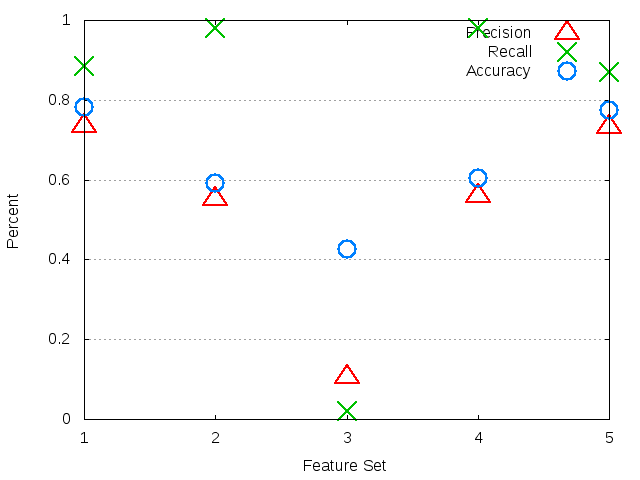
\includegraphics[width=0.8\textwidth]{images/svm/test_3/ShowcaseView_sample_range}
        \caption{Feature for ShowcaseView using \gls{svm}}
        \label{fig:test_3_ShowcaseView_svm-exp}
\end{figure}

\begin{figure}[!ht]
    \centering
        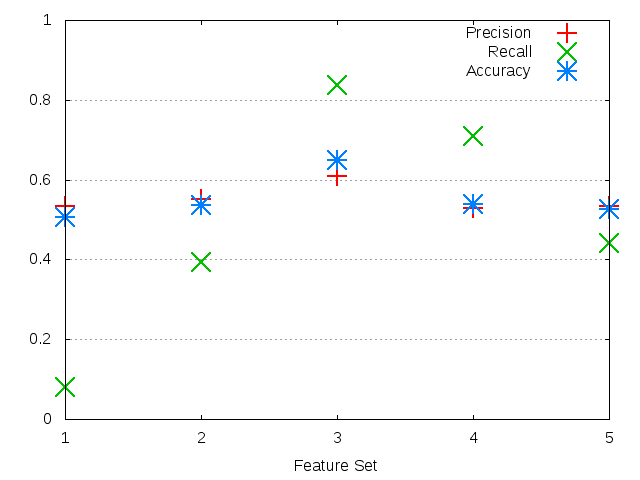
\includegraphics[width=0.8\textwidth]{images/svm/test_3/deeplearning4j_sample_range}
    \caption{Feature for deeplearning4j using \gls{svm}}
    \label{fig:test_3_deeplearning4j_svm-exp}
\end{figure}

\begin{figure}[!ht]
    \centering
        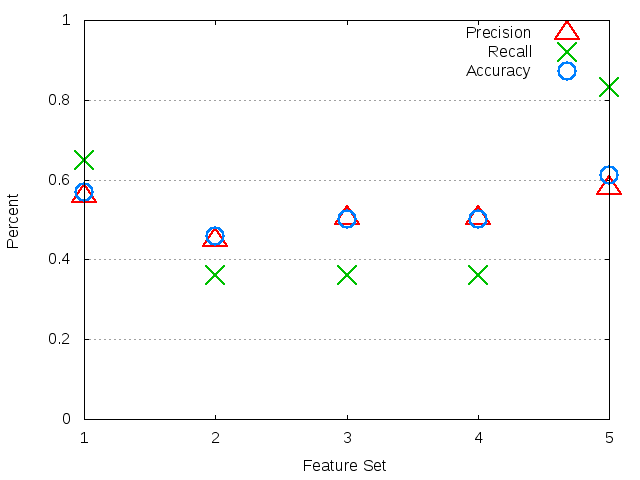
\includegraphics[width=0.8\textwidth]{images/svm/test_3/ion_sample_range}
        \caption{Feature for ion using \gls{svm}}
        \label{fig:test_3_ion_svm-exp}
\end{figure}

The repositories ShowcaseView, deeplearning4j and ion were all greatly impacted by the different feature sets. ShowcaseView in \autoref{fig:test_3_ShowcaseView_svm-exp} performed well for feature set 1 and 5 and terribly for feature set 3. 
Similarly for ion in \autoref{fig:test_3_ion_svm-exp}, feature sets 1 and 5 performed well with the rest of the feature sets performing poorly. Finally for deeplearning4j in \autoref{fig:test_3_deeplearning4j_svm-exp}, the best performance was for feature set 3 where as the remaining trails were not as good. There were a few repositories like these ones were one or two of the feature sets would perform well. One that performed well for certain feature sets tended to share similar repository classifications like ShowcaseView and ion do.

\begin{figure}[!ht]
    \centering
        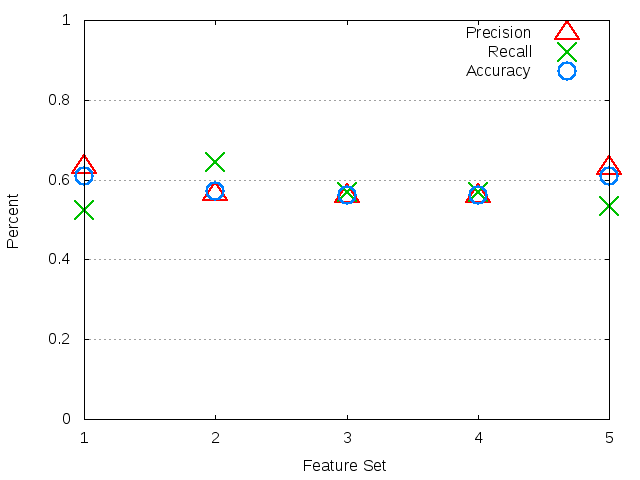
\includegraphics[width=0.8\textwidth]{images/svm/test_3/nettosphere_sample_range}
        \caption{Feature for nettosphere using \gls{svm}}
        \label{fig:test_3_nettosphere_svm-exp}
\end{figure}

\begin{figure}[!ht]
    \centering
        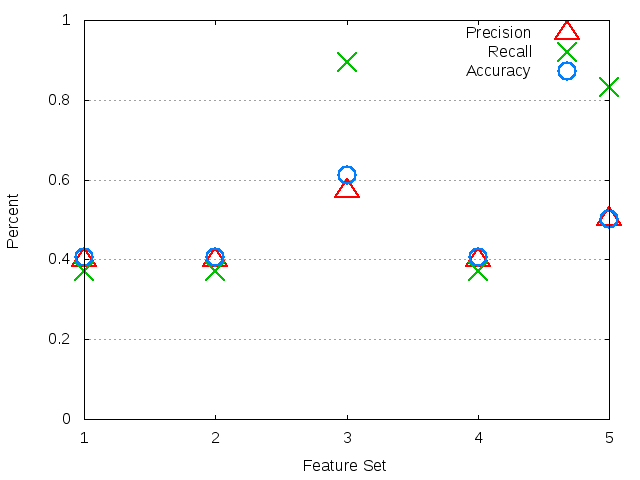
\includegraphics[width=0.8\textwidth]{images/svm/test_3/mapstruct_sample_range}
        \caption{Feature for mapstruct using \gls{svm}}
        \label{fig:test_3_mapstruct_svm-exp}
\end{figure}

\begin{table}
\begin{center}
    \begin{tabular}{|c||c|c||c|c|c|}
        \hline
        \textbf{Repository} & \textbf{AI} & \textbf{Feature} & \textbf{Precision} & \textbf{Recall} & \textbf{Accuracy} \\
         & & \textbf{Set} & & & \\
        \hline
        acra & SVM & 4 & 0.77 & 0.78 & 0.77 \\
        arquillian-core & SVM & 4 & 0.55 & 0.83 & 0.57 \\
        blockly-android & SVM & 2, 3, 4 & 0.5 & 1.0 & 0.5 \\
        brave & SVM & 3, 4 & 0.6 & 0.51 & 0.58 \\
        cardslib & SVM & 5 & 0.51 & 0.88 & 0.52 \\
        dagger & SVM & 1 & 0.51 & 0.9 & 0.52 \\
        deeplearning4j & SVM & 3 & 0.61 & 0.84 & 0.65 \\
        fresco & SVM & 3 & 0.5 & 0.99 & 0.5 \\
        governator & SVM & 1 & 0.65 & 0.57 & 0.63 \\
        greenDAO & SVM & 3, 4 & 0.5 & 1.0 & 0.5 \\
        http-request & SVM & 1 & 0.66 & 0.7 & 0.67 \\
        ion & SVM & 5 & 0.58 & 0.83 & 0.61 \\
        jadx & SVM & 3, 4 & 0.52 & 0.84 & 0.53 \\
        mapstruct & SVM & 3 & 0.57 & 0.9 & 0.61 \\
        nettosphere & SVM & 2 & 0.56 & 0.64 & 0.57 \\
        parceler & SVM & 1 & 0.57 & 0.92 & 0.61 \\
        retrolambda & SVM & 1 & 0.57 & 0.7 & 0.59 \\
        ShowcaseView & SVM & 1 & 0.73 & 0.89 & 0.78 \\
        smile & SVM & 5 & 0.53 & 0.96 & 0.55 \\
        spark & SVM & 2, 4 & 0.5 & 1.0 & 0.5 \\
        storm & SVM & 2 & 0.5 & 0.67 & 0.5 \\
        tempto & SVM & 5 & 0.53 & 0.5 & 0.53 \\
        yardstick & SVM & 3 & 0.53 & 0.68 & 0.54 \\
        \hline
    \end{tabular}
\end{center}
\caption{Feature Repository Best Performance using \gls{svm}}
\label{tab:svm_fs_repository_performance}
\end{table}


A lot of repositories did not vary greatly for different feature sets providing similar to results to that of nettosphere in \autoref{fig:test_3_nettosphere_svm-exp}. All three performance measures show little variance and only small chances are present between repositories. Other repositories performed poorly for all the feature sets such as mapstruct in \autoref{fig:test_3_mapstruct_svm-exp} which had 3 of the 5 trails score lower than $0.5$ in all performance measures. In \autoref{tab:svm_fs_repository_performance} each repository is outlined with the best performance for this experiment. The feature sets are shown to be an influencing factor on the performance of the model however no single feature set found to stand out as the ideal candidate for all repositories.

\subsubsection{SVM Oversampling Experiment}
\label{sec:svm_os_experiment}

% TODO add other tests to this subsection
\begin{table}[h]
\begin{center}

    \begin{tabular}{|c|c|c|c|cc|}
        \hline
        \textbf{Extended} & \textbf{Under} & \textbf{Sample} & \textbf{Window} & \textbf{SVM} & \\
        \textbf{Window} & \textbf{Sampling} & \textbf{Rate} & \textbf{Offset} &  \textbf{C} & \textbf{gamma} \\ \hline
        No & Yes & $100\%$ & 5 & 10 & 8 \\ \hline
    \end{tabular}
    \caption{Feature Experiment Setup}
    \label{tab:rf_feature_experiment_3_setup}
\end{center}

\end{table}


Oversampling is a balancing technique used to increase the amount of samples available. Samples from the smaller data set are re-sampled to increase the size of the data set. While this does introduce duplicates into the model it also counter acts biasing that is present when one classification is more common then the other by a large margin. Under sampling is also used to remove excess elements from the larger set of classification. Oversampling This is especially useful for data sets that contain a small number of samples for a particular category. In that case under sampling may limit the performance of a model by removing nearly all of the elements in the data set.

\begin{table}[ht]
\begin{center}

    \begin{tabular}{|c|c|c|c|c|}
        \hline
        \textbf{Repository} & \multicolumn{2}{c|}{\textbf{Best}} & \multicolumn{2}{c|}{\textbf{Worst}} \\ \cline{2-5}
         & \textbf{Feature Set} & \textbf{SWR} & \textbf{Feature Set} & \textbf{SWR} \\ 
        %Set & & & & & $\Delta_{freq}$ & & & Next \\
        \hline
        acra & 2 & 80 & 3 & 90 \\
        arquillian-core & 4 & 90 & 2 & 90 \\
        blockly-android & 2 & 60 & 2 & 90 \\
        brave & 2 & 130 & 3 & 90 \\
        cardslib & 2 & 120 & 4 & 90 \\
        dagger & 5 & 90 & 2 & 70 \\
        deeplearning4j & 3 & 90 & 2 & 130 \\
        fresco & 3 & 90 & 2 & 90 \\
        governator & 1 & 90 & 3 & 90 \\
        greenDAO & 4 & 90 & 1 & 90 \\
        http-request & 2 & 80 & 3 & 90 \\
        ion & 5 & 90 & 2 & 90 \\
        jadx & 2 & 130 & 2 & 100 \\
        mapstruct & 2 & 70 & 1 & 90 \\
        nettosphere & 2 & 120 & 3 & 90 \\
        parceler & 1 & 90 & 2 & 90 \\
        retrolambda & 2 & 130 & 4 & 90 \\
        ShowcaseView & 1 & 90 & 2 & 80 \\
        smile & 2 & 70 & 2 & 90 \\
        spark & 4 & 90 & 3 & 90 \\
        storm & 2 & 100 & 2 & 110 \\
        tempto & 2 & 120 & 2 & 130 \\
        yardstick & 2 & 70 & 2 & 100 \\


        % acra & 90 & 130 \\
        % dagger & 60 & 70 \\
        % fresco & 130 & 90 \\
        % storm & 80 & 130 \\
        % deeplearning4j & 120 & 130 \\

        \hline
    \end{tabular}
    \caption{Best And Worst Results From experiments 1 and 2 for SVM}
    \label{tab:svm_best_worst_swr_experiment_sets}
\end{center}
\end{table}

The experiment below took the best and worst trials from the previous two experiments and used oversampling when sampling the data. The variables that change per repository are based on the previous best performance and worst performance. In \autoref{tab:svm_best_worst_swr_experiment_sets}, the best and worst \gls{swr} and feature set are provided for each repository. Since each repository will likely have different values of \gls{swr} and feature set the comparesion should only be made between the difference in performance for the best/worst result and their corresponding oversampling trail Best-O/Worst-O.

In some cases the best performing experiment may not have been entirely clear. For example with some repositories having very high recall ($ \geq 0.9$) while having lower precision and accuracy. The best trail was picked based on having the all a weighted summation algorithm outlined in \autoref{eq:repository_ranking_formula}. Since precision and accuracy are very closely related the weight for each was $0.5$ while recall was set to $1.0$.

% Projects to discuss:
% - acra
% - deeplearning4j
% - fresco
% - blockly-android

\begin{figure}[!t]
    \centering
        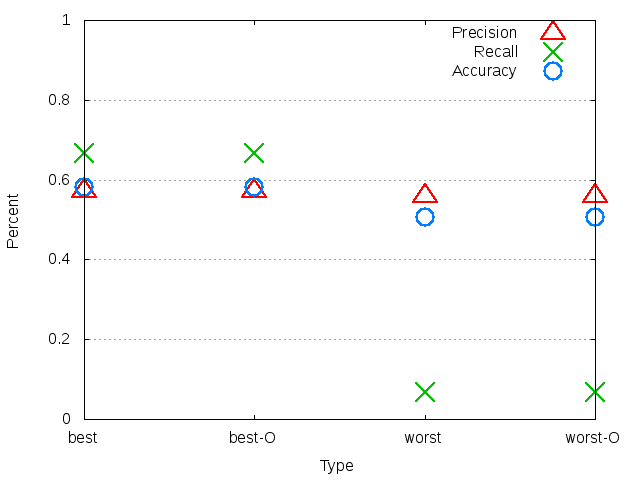
\includegraphics[width=0.8\textwidth]{images/svm/test_4/fresco_sample_range}
        \caption{Oversampling for fresco using \gls{svm}}
        \label{fig:test_4_fresco_svm-exp}
\end{figure}

\begin{figure}[!ht]
    \centering
        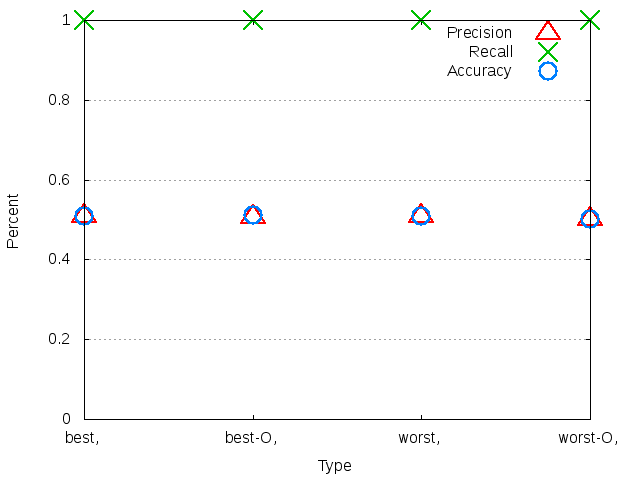
\includegraphics[width=0.8\textwidth]{images/svm/test_4/blockly-android_sample_range}
        \caption{Oversampling for blockly-android using \gls{svm}}
        \label{fig:test_4_blockly-android_svm-exp}
\end{figure}

\begin{figure}[!ht]
    \centering
        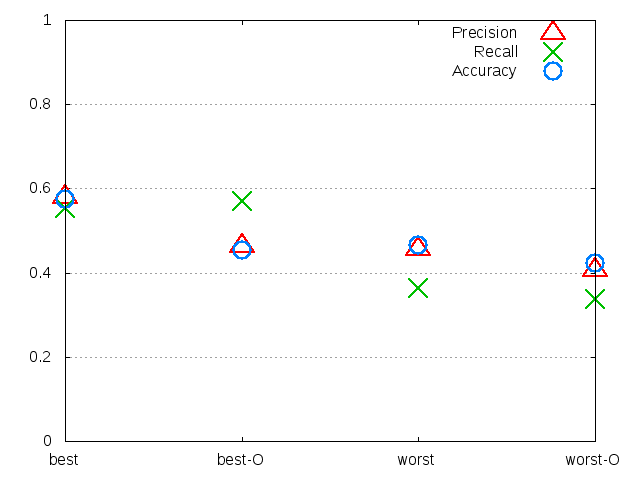
\includegraphics[width=0.8\textwidth]{images/svm/test_4/deeplearning4j_sample_range}
    \caption{Oversampling for deeplearning4j using \gls{svm}}
    \label{fig:test_4_deeplearning4j_svm-exp}
\end{figure}

\begin{figure}[!ht]
    \centering

        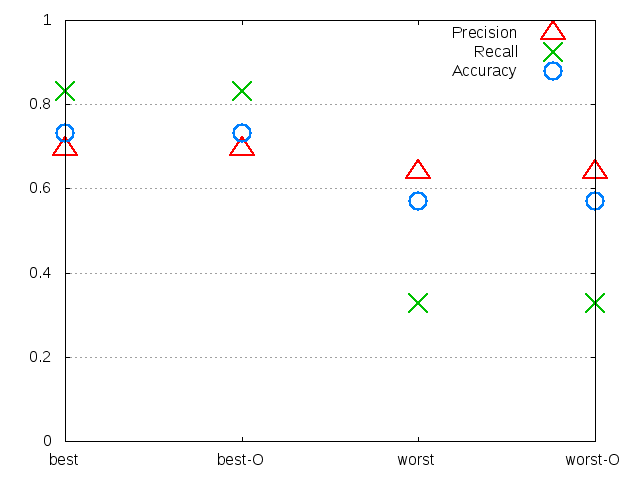
\includegraphics[width=0.8\textwidth]{images/svm/test_4/acra_sample_range}
        \caption{Oversampling for acra using \gls{svm}}
        \label{fig:test_4_acra_svm-exp}
\end{figure}


Some repositories such as fresco \autoref{fig:test_4_fresco_svm-exp} performed a little better for precision and accuracy while a little worse for precision. Unlike most repositories however blockly-android in \autoref{fig:test_4_blockly-android_svm-exp} experienced very little change with the introduction of oversampling. Finally, the majority of the experiments showed oversampling to provide a negative impact of the performance of the model. Both deeplearning4j in \autoref{fig:test_4_deeplearning4j_svm-exp} and acra in \autoref{fig:test_4_acra_svm-exp} performed worse for all measures for both trails.

The overall impact of using oversampling for training the model proved detrimental with the vast majority of repositories performing worse with the use of oversampling. While some repositories experience increases in individual performance measures, other measures fall. Also, any performance seen by a repository is minimal at best while the loss of performance tends to be substantial.

\subsubsection{SVM Discussion}
\label{subsec:svm_discussion}

The three different experiments attempted to determine the impact of the different factors on the prediction method. The three factors that were tested are:
\begin{enumerate}
\item \gls{swr}
\item Model features
\item Sampling balancing
\end{enumerate}

% TODO talk about the performance of the different groups for each experiment
The results of the repositories did not follow any common trends between repositories. Similar repository groups outlined in \autoref{tab:repository_size_summary_info} do not perform similarly for the most part with the exception of the group for acra, dagger and ShowcaseView which all had an okay but for different values of \gls{swr}. The only similarity that can be found is for groups of repository that performed poorly which still was inconsistent. For most repositories at the very least the recall was variable. The only really exception would be blockly-android which experienced little to no variation in for each trial. Some repositories saw more variation in the precision and accuracy and often had at least trail which performed moderately well.

For the second experiment, the performance results were a lot lower than the first generally. This appears to be directly related to the impact that each of these variables has on the performance of the model. Therefore the focus is placed on the best feature set for all repositories or for groups of repositories. For some of the groups of repositories, a certain feature set or pair of feature sets performed well for all repositories in the group. For example, acra, dagger and ShowcaseView all performed well when using feature set 1 or 5. Not all of the repositories performed their best using that those feature sets. However, they did perform close to their best performance. While this trend occurred for some repositories it was not consistent for all repositories. Similarly there was no best performing feature set for all repository.

Finally of the third experiment was found to have a variable impact on the repositories when sample balancing through oversampling was applied. In terms of performance impact, oversampling provide a negative impact on most of the repositories experimented on. Some trials saw now change and a very small number of trails saw slight improvements to one performance measure while decreasing another performance measure. The slight improvements found from using oversampling were insignificant compared to the drop in performance typically experienced.

Overall \gls{swr} had the greatest impact on the performance of the prediction method. The model feature set had less of an impact and balancing the sample through oversampling provided a primarily negative impact. The \gls{swr} while having a larger impact on most repositories, some repositories were less affected. Generally variations of \gls{swr} could produce a positive results, a negative results were also present. Furthermore, no clear pattern was discovered to allow for simple configuration of the parameters to provide positive results. Therefore use of the approach with a \gls{svm} model can be beneficial but also incurs a risk associated with poor predictions.

\subsection{Random Forest Experiments}
\label{sec:rf_experiments}

The machine learning algorithm \gls{rf} is used for the second set of experiments. \gls{rf} was selected as an alternative to \gls{svm} for it's success in various data mining related tools. The implementation of \gls{rf} is in a python library \textit{scikit-learn} which is outlined in \Cref{sec:prediction_method}. Only one parameter is used for \gls{rf}, the forest size, which is set to $10000$ all of these experiments.

\subsubsection{Window Range Experiments}
\label{sec:rf_swr_experiment}

\begin{table}[h]
\begin{center}

    \begin{tabular}{|c|c|c|c|c|c|c|c|}
        \hline
        Com & Sig & Name & $f_{\Delta}$ & $sf_{\Delta}$ & $t_\Delta$ & Length & $change_{t-1}$ \\
        %Set & & & & & $\Delta_{freq}$ & & & Next \\
         \hline
        $\bullet$ & $\bullet$ & $\bullet$ & $\bullet$ & & $\bullet$ & $\bullet$ & $\bullet$ \\ \hline
    \end{tabular}
    \caption{\gls{swr} Experiment Features}
    \label{tab:rf_window_range_experiment_features}
\end{center}

\end{table}

\begin{table}[h]
\begin{center}

    \begin{tabular}{|c|c|c|c|c|c|}
        \hline
        \textbf{Extended} & \textbf{Over} & \textbf{Under} & \textbf{Sample} & \textbf{Window} & \textbf{RF} \\
        \textbf{Window} & \textbf{Sampling} & \textbf{Sampling} & \textbf{Rate} & \textbf{Offset} & \textbf{Size} \\ \hline
        No & No & Yes & $100\%$ & 5 & 10000 \\ \hline
    \end{tabular}
    \caption{\gls{swr} Experiment Setup}
    \label{tab:rf_window_range_experiment_setup}
\end{center}

\end{table}

The independent variable for this set of experiments is the sample window size measured in commits. The feature set are outlined in \autoref{tab:rf_window_range_experiment_features}. The features used for this experiment is the same as the first \gls{svm} experiment feature set.

The parameters for this experiment are outlined in \autoref{tab:rf_window_range_experiment_setup}. The only difference between the parameters used in this experiment and the parameters used in the \gls{svm} experiment one is the \gls{rf} specific parameters. This allows for a fairly clear comparison between these two methods with the given independent variable, the \gls{swr}. The experiment was conducted on all 23 repositories collected and examples were are discussed in more detail in this section. The remainder of the repositories performance results are outlined in \autoref{app_sub:experiment_1_rf}.

% Projects
% http-request
% jadx
% parceler
% storm
% dagger

\begin{figure}[!ht]
    \centering

        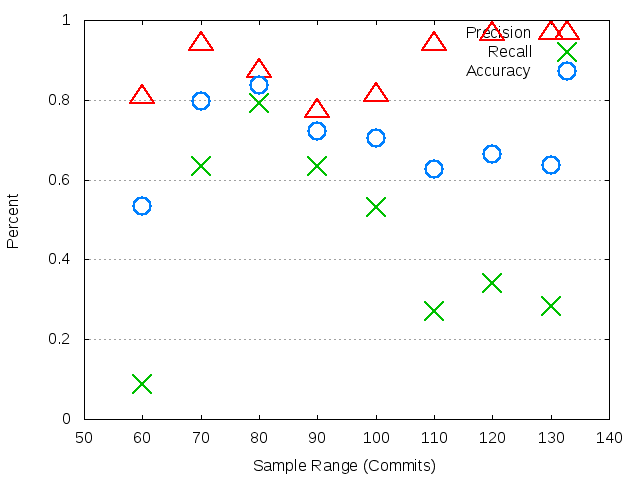
\includegraphics[width=0.8\textwidth]{images/rf/test_1/http-request_sample_range}
        \caption{\gls{swr} for http-request using \gls{rf}}
        \label{fig:test_1_http-request_rf-exp}

    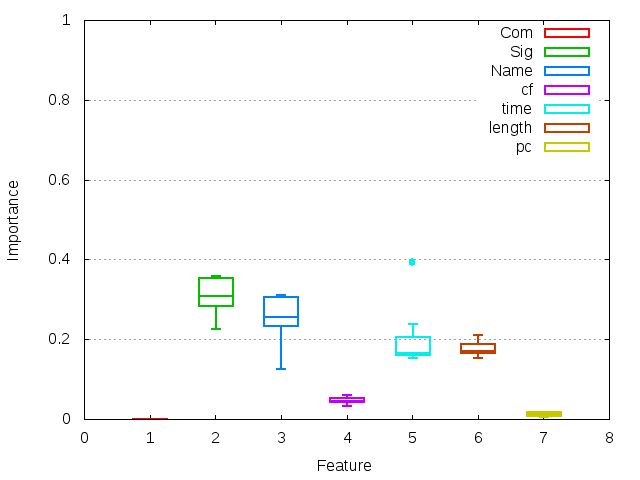
\includegraphics[width=0.8\textwidth]{images/rf/test_1/http-request_importance}
        \caption{Feature Importance \gls{swr} for http-request using \gls{rf}}
        \label{fig:test_1_http-request_rf_importance-exp}
\end{figure}

\begin{figure}[!ht]
    \centering
        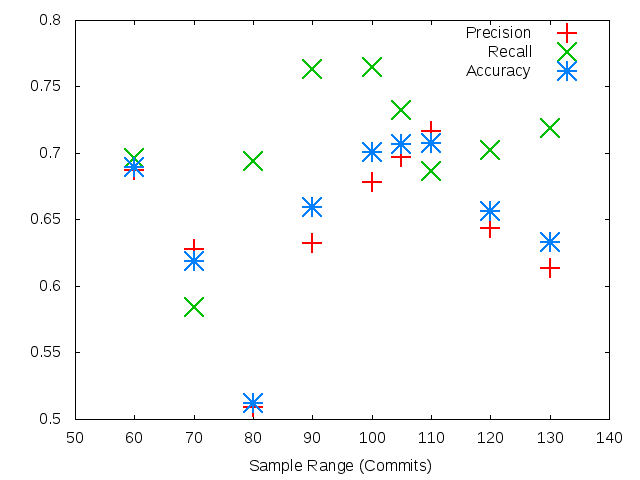
\includegraphics[width=0.8\textwidth]{images/rf/test_1/dagger_sample_range}
        \caption{\gls{swr} for dagger using \gls{rf}}
        \label{fig:test_1_dagger_rf-exp}

    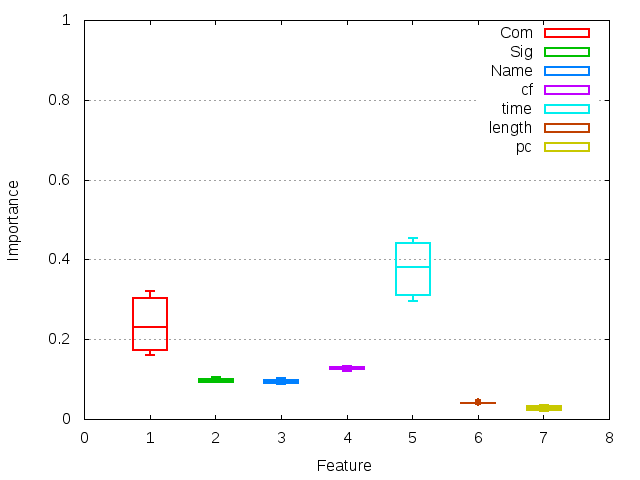
\includegraphics[width=0.8\textwidth]{images/rf/test_1/dagger_importance}
        \caption{Feature Importance \gls{swr} for dagger using \gls{rf}}
        \label{fig:test_1_dagger_rf_importance-exp}
\end{figure}

Each repositories experimental results are accompanied with a second figure that outlines the importance for each feature set variable in the creation of the prediction model. The importance of a feature only identifies how influential that feature was to the prediction and therefore necessitates the context of the results. So if a repository performs poorly in predicting the most influential features are more likely to not as useful for predictions with the repository. Likewise, if a repository performs well the corresponding feature importance can indicate highly influential features that helped produce positive results.

Even in the case of where a repository performs well the feature set used may not be generalizable to other repositories. For example http-request in \autoref{fig:test_1_http-request_rf_importance-exp} performs well with a \gls{swr} of 70 - 90 and places high importance on $Sig$, $Name$, $time$ and $length$. Alternatively, dagger in \autoref{fig:test_1_dagger_rf_importance-exp} performs moderately well with an \gls{swr} of 60 and 100-110 while placing a higher importance on $Com$ and $time$. Even more interesting is that http-request placed nearly 0 importance on $Com$ while the same feature ranked second for dagger.

\begin{figure}[!ht]
    \centering
        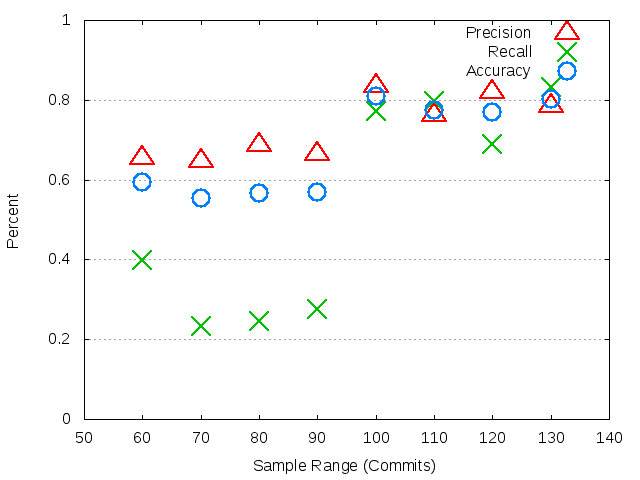
\includegraphics[width=0.8\textwidth]{images/rf/test_1/ShowcaseView_sample_range}
        \caption{\gls{swr} for ShowcaseView using \gls{rf}}
        \label{fig:test_1_ShowcaseView_rf-exp}

    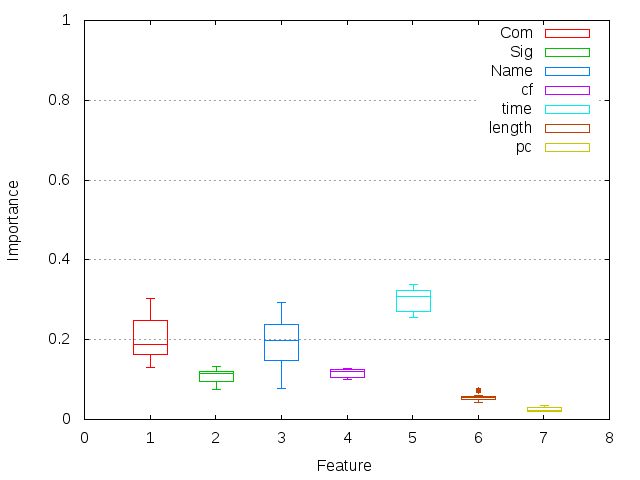
\includegraphics[width=0.8\textwidth]{images/rf/test_1/ShowcaseView_importance}
        \caption{Feature Importance \gls{swr} for ShowcaseView using \gls{rf}}
        \label{fig:test_1_ShowcaseView_rf_importance-exp}
\end{figure}

\begin{figure}[!ht]
    \centering
        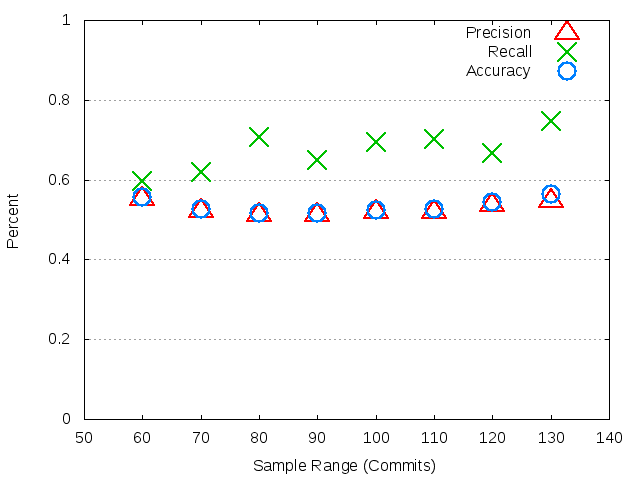
\includegraphics[width=0.8\textwidth]{images/rf/test_1/jadx_sample_range}
    \caption{\gls{swr} for jadx using \gls{rf}}
    \label{fig:test_1_jadx_rf-exp}

    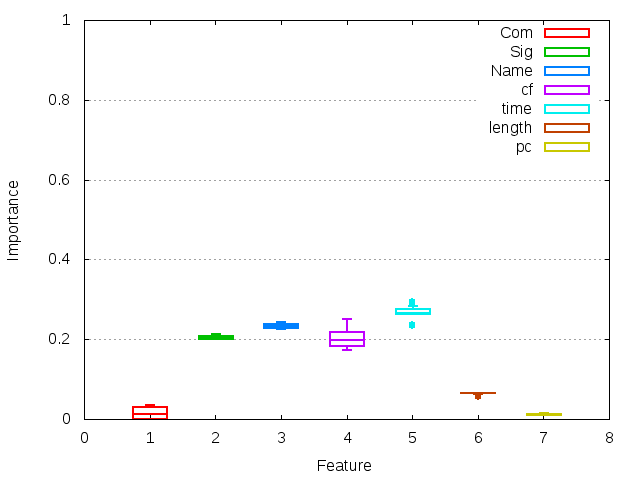
\includegraphics[width=0.8\textwidth]{images/rf/test_1/jadx_importance}
        \caption{Feature Importance \gls{swr} for jadx using \gls{rf}}
        \label{fig:test_1_jadx_rf_importance-exp}
\end{figure}

The performance of each repository varied, with a few repositories performing well for some \gls{swr} like http-request in \autoref{fig:test_1_http-request_rf-exp}, dagger in \autoref{fig:test_1_dagger_rf-exp} and ShowcaseView in \autoref{fig:test_1_ShowcaseView_rf-exp}. The impact of the changes to \gls{swr} is clearly visible as some trails perform poorly, while others perform a lot better. For example in ShowcaseView, use of a \gls{swr} of 100 or higher provides good performance but below the performance is a lot lower. For some repositories such as jadx in \autoref{fig:test_1_jadx_rf-exp} the \gls{swr} had less of an impact causing little variation between precision and accuracy while offering only slight changes with the recall.

\begin{figure}[!ht]
    \centering
        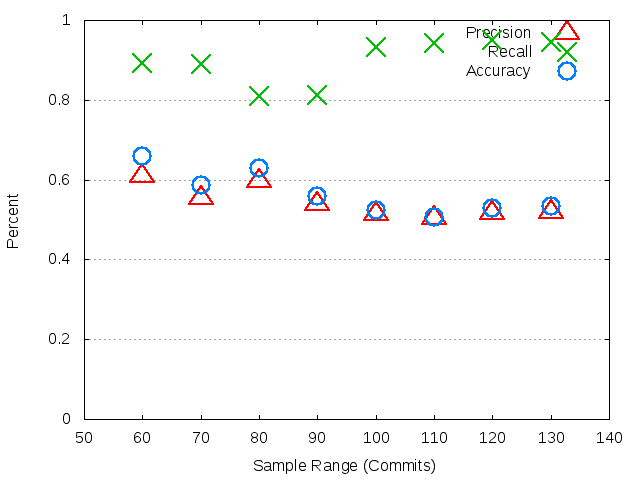
\includegraphics[width=0.8\textwidth]{images/rf/test_1/storm_sample_range}
        \caption{\gls{swr} for storm using \gls{rf}}
        \label{fig:test_1_storm_rf-exp}

    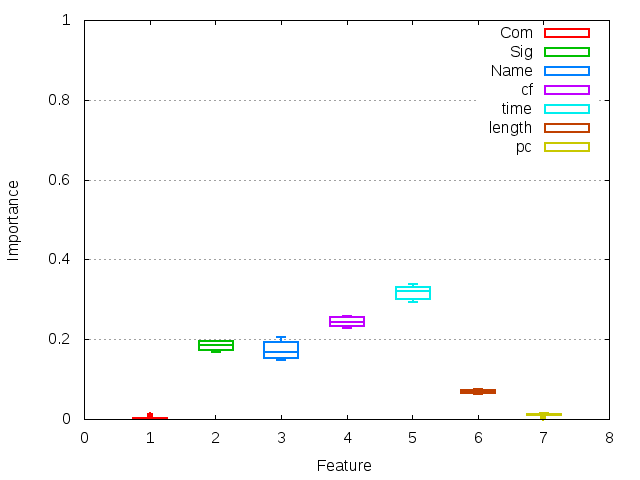
\includegraphics[width=0.8\textwidth]{images/rf/test_1/storm_importance}
        \caption{Feature Importance \gls{swr} for storm using \gls{rf}}
        \label{fig:test_1_storm_rf_importance-exp}
\end{figure}

\begin{figure}[!t]
    \centering
        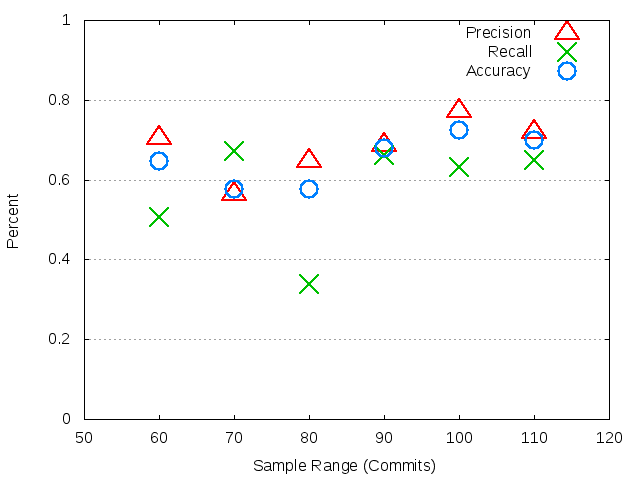
\includegraphics[width=0.8\textwidth]{images/rf/test_1/parceler_sample_range}
        \caption{\gls{swr} for parceler using \gls{rf}}
        \label{fig:test_1_parceler_rf-exp}

    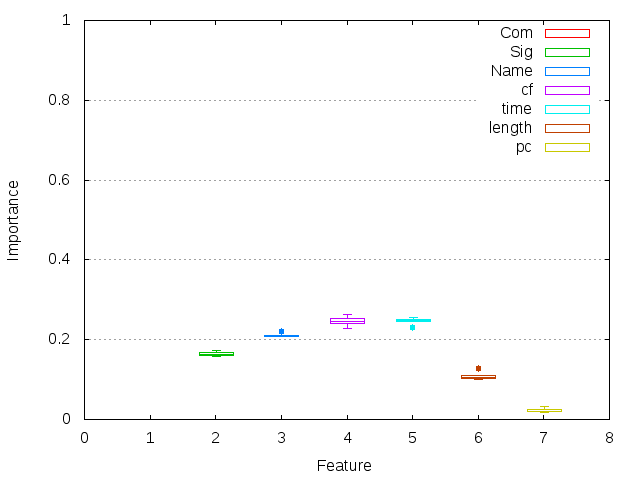
\includegraphics[width=0.8\textwidth]{images/rf/test_1/parceler_importance}
        \caption{Feature Importance \gls{swr} for parceler using \gls{rf}}
        \label{fig:test_1_parceler_rf_importance-exp}
\end{figure}

\begin{table}
\begin{center}
    \begin{tabular}{|c||c|c||c|c|c|}
        \hline
        \textbf{Repository} & \textbf{AI} & \textbf{SWR} & \textbf{Precision} & \textbf{Recall} & \textbf{Accuracy} \\
        % & & \textbf{Set} & & & \\
        \hline
        acra & RF & 90 & 0.78 & 0.75 & 0.77 \\
        arquillian-core & RF & 90 & 0.52 & 0.98 & 0.54 \\
        blockly-android & RF & 70 & 0.59 & 0.65 & 0.6 \\
        brave & RF & 90 & 0.6 & 0.95 & 0.65 \\
        cardslib & RF & 100 & 0.65 & 0.74 & 0.67 \\
        dagger & RF & 110 & 0.72 & 0.69 & 0.71 \\
        deeplearning4j & RF & 120 & 0.57 & 0.93 & 0.61 \\
        fresco & RF & 60 & 0.52 & 1.0 & 0.53 \\
        governator & RF & 60 & 0.57 & 0.81 & 0.6 \\
        greenDAO & RF & 120 & 0.54 & 0.54 & 0.54 \\
        http-request & RF & 80 & 0.87 & 0.79 & 0.84 \\
        ion & RF & 90 & 0.71 & 0.73 & 0.72 \\
        jadx & RF & 130 & 0.55 & 0.75 & 0.56 \\
        mapstruct & RF & 110 & 0.58 & 0.88 & 0.62 \\
        nettosphere & RF & 110 & 0.63 & 0.67 & 0.63 \\
        parceler & RF & 100 & 0.77 & 0.63 & 0.72 \\
        retrolambda & RF & 70 & 0.56 & 0.73 & 0.58 \\
        ShowcaseView & RF & 130 & 0.78 & 0.83 & 0.8 \\
        smile & RF & 100 & 0.53 & 0.84 & 0.54 \\
        spark & RF & 110 & 0.54 & 0.91 & 0.57 \\
        storm & RF & 60 & 0.61 & 0.89 & 0.66 \\
        tempto & RF & 70 & 0.58 & 0.65 & 0.59 \\
        yardstick & RF & 70 & 0.54 & 0.67 & 0.55 \\
        \hline
    \end{tabular}
\end{center}
\caption{\gls{swr} Repository Best Performance using \gls{rf}}
\label{tab:rf_swr_repository_performance}
\end{table}

In \autoref{tab:rf_swr_repository_performance}, the best performance is shown for each repository for this experiment. Some repositories experienced very little impact from variations of the \gls{swr} for the performance. For example, storm in \autoref{fig:test_1_storm_rf-exp} had higher recall but lower precision and accuracy. Other factors may provide more influence such smaller or larger values of \gls{swr} however those were outside the scope of the experiment. Finally, other repositories did not perform as well but experienced some variation to precision, recall and accuracy. One such repository would be \autoref{fig:test_1_parceler_rf-exp} which had all three measures fairly close together for most trails but because of the size of the repository could not supply sufficient data for a \gls{swr} of 120 or 130. The importance of both storm and parceler was similar to that of http-request however as noted neither managed to perform as well as the best performance from http-request.

\subsubsection{Feature Set Experiments}
\label{sec:feature_set_experiment_rf}

\begin{table}[h]
\begin{center}

    \begin{tabular}{|c|c|c|c|c|c|c|}
        \hline
        \textbf{Extended} & \textbf{Over} & \textbf{Under} & \textbf{Sample} & \textbf{Window} & \textbf{SWR} & \textbf{RF} \\
        \textbf{Window} & \textbf{Sampling} & \textbf{Sampling} & \textbf{Rate} & \textbf{Offset} &  & \textbf{Size} \\ \hline
        No & No & Yes & $100\%$ & 5 & 90 & 10000 \\ \hline
    \end{tabular}
    \caption{Candidate Feature Experiment Setup}
    \label{tab:rf_feature_experiment_setup}
\end{center}

\end{table}



%The parameter for this experiment are outlined in \autoref{tab:window_range_experiment_setup}. The major difference between the \gls{svm} and this experiment, \gls{rf}, is the parameters used for the \gls{rf}. This allows for a fairly clear comparison between these two methods with the given independent variable, sample window size.

\begin{table}[h]
\begin{center}

    \begin{tabular}{|c|c|c|c|c|c|c|c|c|}
        \hline
        Feature & Com & Sig & Name & $f_{\Delta}$ & $sf_{\Delta}$ & $t_\Delta$ & Length & $change_{t-1}$ \\
        %Set & & & & & $\Delta_{freq}$ & & & Next \\
         \hline
        1 & $\bullet$ & $\bullet$ & $\bullet$ & $\bullet$ & $\bullet$ & & $\bullet$ & $\bullet$ \\
        2 & $\bullet$ & $\bullet$ & $\bullet$ & $\bullet$ & & $\bullet$ & $\bullet$ & $\bullet$ \\
        3 & $\bullet$ & $\bullet$ & $\bullet$ & $\bullet$ & & $\bullet$ & & $\bullet$ \\
        4 & & $\bullet$ & $\bullet$ & $\bullet$ & & $\bullet$ & & $\bullet$ \\
        5 & $\bullet$ & $\bullet$ & $\bullet$ & $\bullet$ & & & & $\bullet$ \\ \hline
        %6 & $\bullet$ & & & & $\bullet$ & $\bullet$ & $\bullet$ & \\ 
    \end{tabular}
    \caption{Candidate Feature Sets}
    \label{tab:rf_feature_experiment_sets}
\end{center}

\end{table}

% Projects:
% cardslib (example of project that had basically no difference in performance)
% governator (example of a project that did terrible for each)
% ShowcaseView (performed really well)
% dagger (variable performance)
% ion high all around performance

Similar to the experiment using a \gls{svm} in \Cref{sec:svm_feature_set_experiments}. The experiment parameters are outlined in \autoref{tab:rf_feature_experiment_setup}. The candidate features are likewise outlined in \autoref{tab:rf_feature_experiment_sets}. Each set is assigned an index value to allow for easier reference later on in this section. The candidate feature set will be referenced by the index assigned in the plots and discussions related. The candidate feature sets were used experimented on with each repository which are discussed below. The following results are highlights of the larger set of experiments conducted on each repository. The remainder of the results for this experiment are outlined in \autoref{app_sub:experiment_2_rf}.

\begin{figure}[!ht]
    \centering
        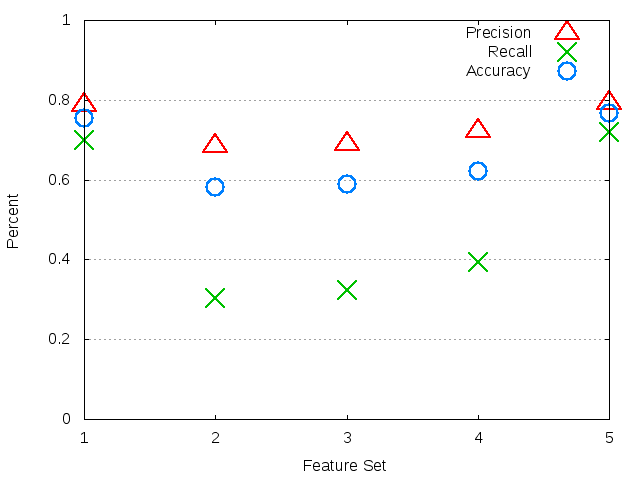
\includegraphics[width=0.8\textwidth]{images/rf/test_3/ShowcaseView_sample_range}
        \caption{Feature for ShowcaseView using \gls{rf}}
        \label{fig:test_3_ShowcaseView_rf-exp}
\end{figure}

\begin{figure}[!ht]
    \centering
        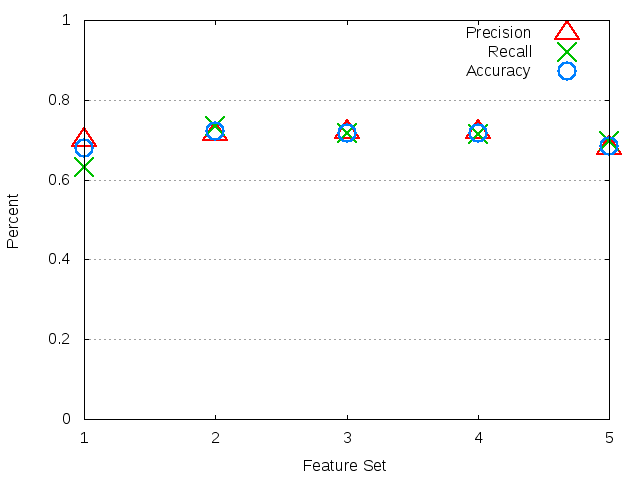
\includegraphics[width=0.8\textwidth]{images/rf/test_3/ion_sample_range}
    \caption{Feature for ion using \gls{rf}}
    \label{fig:test_3_ion_rf-exp}
\end{figure}

\begin{figure}[!ht]
    \centering
        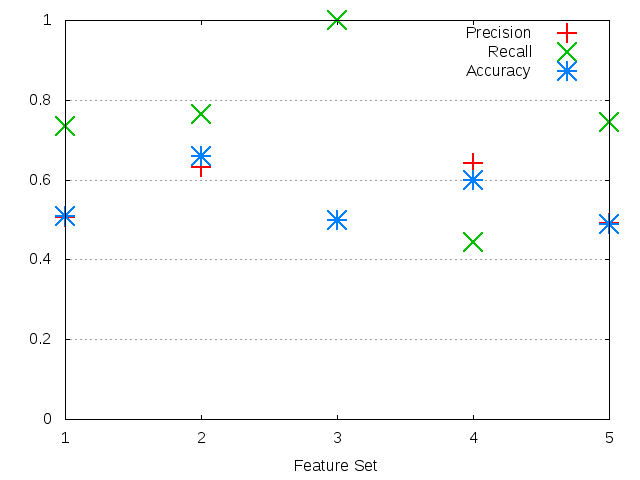
\includegraphics[width=0.8\textwidth]{images/rf/test_3/dagger_sample_range}
        \caption{Feature for dagger using \gls{rf}}
        \label{fig:test_3_dagger_rf-exp}
\end{figure}

The repository to perform the best in this experiment was ShowcaseView in \autoref{fig:test_3_ShowcaseView_rf-exp} which performed best for feature sets 1 and 5 and had minimal difference between the performance of feature sets 2, 3 and 4. Typically most repositories performed well with two feature sets or more which most likely is related to the similarity in the feature sets tested. A few of the successful repositories, such as ion in \autoref{fig:test_3_ion_rf-exp}, performed well consistently for each feature set. Finally, other more successful repositories saw dramatic variations between the different feature sets. For example, dagger in \autoref{fig:test_3_dagger_rf-exp}, performs well in the second feature set and poorly in the rest. The recall is especially volatile at dropping below $0.5$ for feature set 4. 


\begin{figure}[!ht]
    \centering
        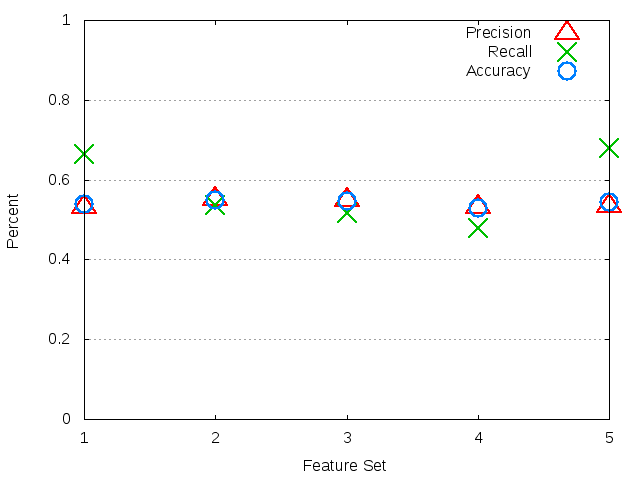
\includegraphics[width=0.8\textwidth]{images/rf/test_3/cardslib_sample_range}
        \caption{Feature for cardslib using \gls{rf}}
        \label{fig:test_3_cardslib_rf-exp}
\end{figure}

\begin{figure}[!ht]
    \centering
        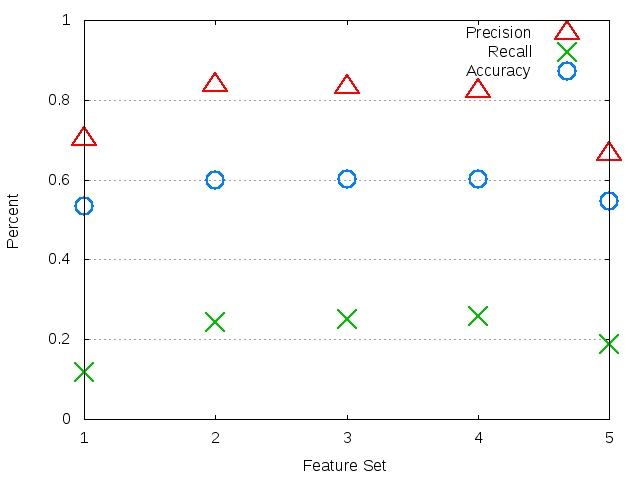
\includegraphics[width=0.8\textwidth]{images/rf/test_3/governator_sample_range}
    \caption{Feature for governator using \gls{rf}}
    \label{fig:test_3_governator_rf-exp}
\end{figure}

\begin{table}
\begin{center}
    \begin{tabular}{|c||c|c||c|c|c|}
        \hline
        \textbf{Repository} & \textbf{AI} & \textbf{Feature} & \textbf{Precision} & \textbf{Recall} & \textbf{Accuracy} \\
         & & \textbf{Set} & & & \\
        \hline
        acra & RF & 4 & 0.77 & 0.78 & 0.77 \\
        arquillian-core & RF & 5 & 0.53 & 0.97 & 0.56 \\
        blockly-android & RF & 2 & 0.56 & 0.73 & 0.58 \\
        brave & RF & 2 & 0.53 & 0.92 & 0.55 \\
        cardslib & RF & 5 & 0.53 & 0.68 & 0.54 \\
        dagger & RF & 2 & 0.63 & 0.76 & 0.66 \\
        deeplearning4j & RF & 3 & 0.54 & 0.91 & 0.56 \\
        fresco & RF & 3 & 0.5 & 1.0 & 0.5 \\
        governator & RF & 3 & 0.83 & 0.25 & 0.6 \\
        greenDAO & RF & 3 & 0.52 & 0.47 & 0.52 \\
        http-request & RF & 1 & 0.67 & 0.7 & 0.68 \\
        ion & RF & 2 & 0.72 & 0.73 & 0.72 \\
        jadx & RF & 3 & 0.51 & 0.67 & 0.52 \\
        mapstruct & RF & 1 & 0.54 & 0.95 & 0.57 \\
        nettosphere & RF & 5 & 0.76 & 0.42 & 0.64 \\
        parceler & RF & 3 & 0.68 & 0.7 & 0.69 \\
        retrolambda & RF & 1 & 0.59 & 0.17 & 0.53 \\
        ShowcaseView & RF & 5 & 0.79 & 0.72 & 0.77 \\
        smile & RF & 4 & 0.51 & 0.85 & 0.52 \\
        spark & RF & 1 & 0.52 & 0.72 & 0.52 \\
        storm & RF & 5 & 0.54 & 0.85 & 0.57 \\
        tempto & RF & 4 & 0.51 & 0.67 & 0.52 \\
        yardstick & RF & 2 & 0.62 & 0.24 & 0.55 \\
        \hline
    \end{tabular}
\end{center}
\caption{Feature Repository Best Performance using \gls{rf}}
\label{tab:rf_fs_repository_performance}
\end{table}

The majority of the repositories experimented on saw little difference for each feature set. The best performance for each repository is outlined in \autoref{tab:rf_fs_repository_performance}. For cardslib in \autoref{fig:test_3_cardslib_rf}, the precision and accuracy stay right above $0.5$ while the recall dips below $0.5$ for feature set 4. The performance is not great and overall the impact of the different feature sets appears quite low for this repository. Alternatively, governator in \autoref{fig:test_3_governator_rf}, is one of the few repositories to perform well for precision while low for accuracy and very low for recall. Each feature set again has only a small impact on the performance with the repository performing very poorly for every trial. Overall the results for this experiment were mixed since the impact of the feature set at least of these three features is less significant that the \gls{swr}.

\subsubsection{Oversampling Experiment}
\label{sec:oversampling_experiment_rf}

\begin{table}[h]
\begin{center}

    \begin{tabular}{|c|c|c|c|c|}
        \hline
        \textbf{Extended} & \textbf{Under} & \textbf{Sample} & \textbf{Window} & \textbf{RF} \\
        \textbf{Window} & \textbf{Sampling} & \textbf{Rate} & \textbf{Offset} & \textbf{Size} \\ \hline
        No & Yes & $100\%$ & 5 & 10000 \\ \hline
    \end{tabular}
    \caption{Oversampling Experiment Setup}
    \label{tab:rf_os_experiment_setup}
\end{center}

\end{table}


This experiment builds on top of the previous two experiments and shares a very similar setup to those experiments.The experiment parameters are outlined in \autoref{tab:rf_os_experiment_setup}. The best and worst trails for each repository are taken from the previous two experiments. The value for \gls{swr} and the feature set used were recorded in \autoref{tab:rf_best_worst_swr_experiment_sets} for each repository for the best and worst performance of the \gls{rf} model. The experiment applies oversampling the best and worst trials to compare the performance of the model with and without the use of oversampling.

\begin{table}[ht]
\begin{center}

    \begin{tabular}{|c|c|c|c|c|}
        \hline
        \textbf{Repository} & \multicolumn{2}{c|}{\textbf{Best}} & \multicolumn{2}{c|}{\textbf{Worst}} \\ \cline{2-5}
         & \textbf{Feature Set} & \textbf{SWR} & \textbf{Feature Set} & \textbf{SWR} \\ 
        %Set & & & & & $\Delta_{freq}$ & & & Next \\
        \hline
        acra & 2 & 60 & 5 & 90 \\
        arquillian-core & 3 & 90 & 4 & 90 \\
        blockly-android & 2 & 90 & 1 & 90 \\
        brave & 2 & 110 & 4 & 90 \\
        cardslib & 2 & 100 & 4 & 90 \\
        dagger & 3 & 90 & 2 & 80 \\
        deeplearning4j & 2 & 70 & 2 & 80 \\
        fresco & 2 & 60 & 2 & 90 \\
        governator & 2 & 60 & 2 & 90 \\
        greenDAO & 2 & 60 & 2 & 100 \\
        http-request & 2 & 80 & 4 & 90 \\
        ion & 2 & 90 & 1 & 90 \\
        jadx & 2 & 130 & 2 & 70 \\
        mapstruct & 1 & 90 & 5 & 90 \\
        nettosphere & 2 & 110 & 2 & 90 \\
        parceler & 3 & 90 & 1 & 90 \\
        retrolambda & 2 & 120 & 2 & 90 \\
        ShowcaseView & 2 & 130 & 2 & 90 \\
        smile & 5 & 90 & 2 & 100 \\
        spark & 2 & 110 & 2 & 80 \\
        storm & 2 & 60 & 2 & 90 \\
        tempto & 2 & 120 & 2 & 130 \\
        yardstick & 2 & 70 & 2 & 60 \\
        % acra & 90 & 130 \\
        % dagger & 90 & 80 \\
        % fresco & 60 & 70 \\
        % storm & 60 & 70 \\
        % deeplearning4j & 100 & 80 \\
        \hline
    \end{tabular}
    \caption{Best And Worst Results From Experiments 1 and 2 for RF}
    \label{tab:rf_best_worst_swr_experiment_sets}
\end{center}
\end{table}

The result of a trail with oversampling are represented in the figures by either \textit{best-O} or \textit{worst-O}. The results without oversampling from the previous experiment are represented with \textit{best} and \textit{worst}.

% Projects to show:
% - arquillian-core (very slight change for the worse)
% - dagger (marginal improvement for best)
% - yardstick (slight overall improvement for best)
% - greenDAO (decrease in performance for worst no change for best)
% - all the rest are pretty much similar to these three with basically no change.

\begin{figure}[!ht]
    \centering
        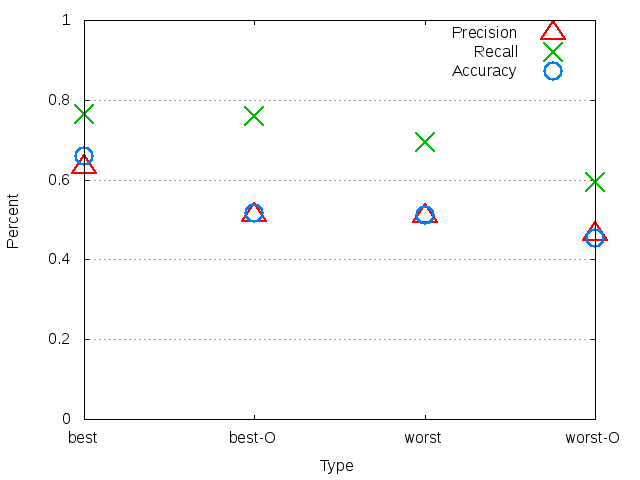
\includegraphics[width=0.8\textwidth]{images/rf/test_4/dagger_sample_range}
        \caption{Oversampling for dagger using \gls{rf}}
        \label{fig:test_4_dagger_rf-exp}
\end{figure}

\begin{figure}[!ht]
    \centering
        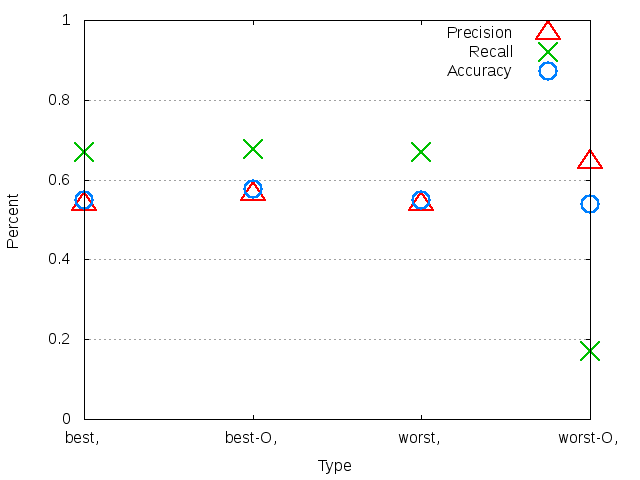
\includegraphics[width=0.8\textwidth]{images/rf/test_4/yardstick_sample_range}
        \caption{Oversampling for yardstick using \gls{rf}}
        \label{fig:test_4_yardstick_rf-exp}
\end{figure}

\begin{figure}[!ht]
    \centering
        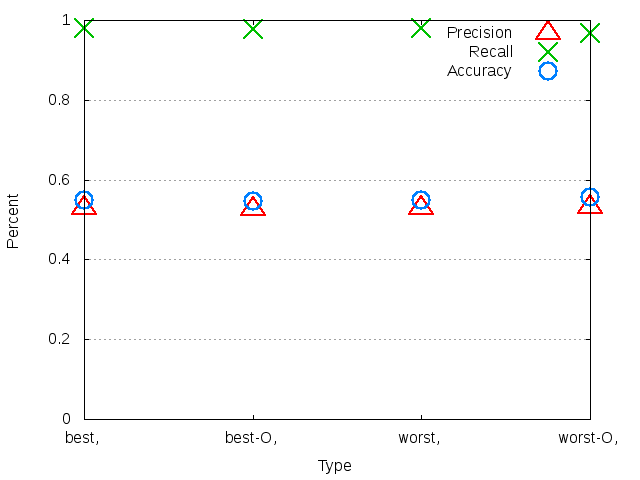
\includegraphics[width=0.8\textwidth]{images/rf/test_4/arquillian-core_sample_range}
        \caption{Oversampling for arquillian-core using \gls{rf}}
        \label{fig:test_4_arquillian-core_rf-exp}
\end{figure}

\begin{figure}[!ht]
    \centering
        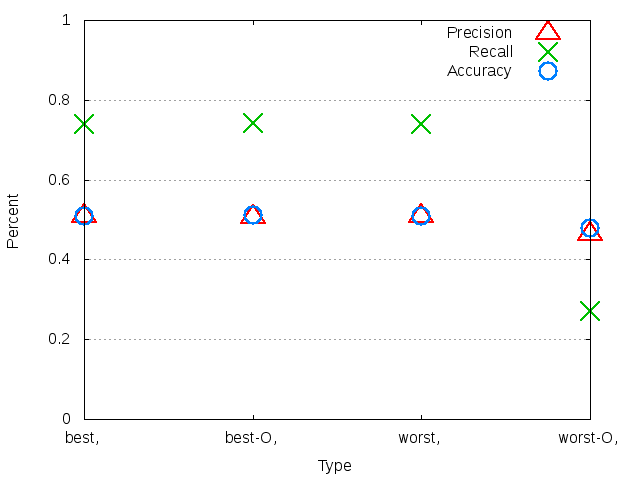
\includegraphics[width=0.8\textwidth]{images/rf/test_4/greenDAO_sample_range}
    \caption{Oversampling for greenDAO using \gls{rf}}
    \label{fig:test_4_greenDAO_rf-exp}
\end{figure}

The results for the use of oversampling on the best and worst trails from each repository provide to have little effect on the results. In rare cases such as dagger in \autoref{fig:test_4_dagger_rf-exp}, the performance marginally improved for the some measures while decreasing for others. However dagger also performed worse when oversampling was used on the worst trial. Similarly yardstick in \autoref{fig:test_4_yardstick_rf-exp}, performed slightly better for best-O and dramatically worse for worst-O.

The majority of the repositories however saw no improvement or a slight decrease in performance. For example arquillian-core in \autoref{fig:test_4_arquillian-core_rf-exp} performed around the same for best-O and slightly worse for worst-O. Generally the differences if any were very small for most. Finally, some repositories performed a lot worse for their worst-O trial including greenDAO in \autoref{fig:test_4_greenDAO_rf-exp}. Overall the use of oversampling on either the best or worst case cause little difference. The only major difference was for worst-O which typically performed poor in compared to the trial without the use of oversampling.

\subsubsection{Random Forest Discussion}
\label{subsec:rf_discussion}

The approach was experimented on using the machine learning algorithm \gls{rf}. The three factors; \gls{swr}, feature set and oversampling were investigated. The first factor, \gls{swr}, achieved positive results for some of the repositories and appeared to have the largest impact on the performance. While the impact of the \gls{swr} was larger often the best result for a repository would of accuracy and precision at $0.5$ and recall at $1.0$. The impact of the feature set should also not be overshadowed as some repositories performed better in the third experiment than the first. Finally, the impact of sample balancing on the data set proved primarily negative with both the best and worst trails performing worse when oversampling was used.

The first experimental results did not show a pattern for present for all the repositories. Some repositories performed better while a lot performed mediocre at just above $0.5$ precision, accuracy. A few of the repositories had poor performances with measures dropping below $0.5$. Most of the groups yielded positive similar results, with acra, dagger and ShowcaseView all performing well and having fairly large variations for different trials. Likewise, aqruillian-core, brave and spark all performed similarly. While the results for these three repository were not particularly good they still showed similar trends of performance.

For the second experiment no particular feature set was found to work for all repositories. Some repositories performed well for some while others performed well for others. Generally though, repositories tended not perform well for all feature sets. One repository such repository to perform poorly was governator which performed well for precision, okay for accuracy and terribly for recall. However in terms of repository groupings, the grouping of acra, dagger and ShowcaseView all performed well but varied in which feature set they performed well with. Overall groups tended to perform differently and had success with different feature sets. A feature set that worked well for one repository in the group could just as easily work poorly for another. This is highlighted best in the group consisting of http-request, nettosphere, parceler and retrolamdba. Both http-request and parceler perform well and nettosphere and retrolamdba perform for badly all feature sets.

Of course the final experiment with oversampling performed similar to the \gls{svm} experiments. For most repositories the use of oversampling in balancing the sample data provided no difference in model performance. The second most common outcome was for trails that used oversampling to result in lower performance than without. Finally in some rare cases, 2 of the 23 repositories saw a one of their trials perform slightly better with the use of oversampling. The results were not consistent for these repositories since the first repository was dagger saw the other corresponding trail decrease in performance. However the second repository, smile, recorded no difference in result for the corresponding trail.

Overall for the experiments using \gls{rf}, the variable with the greatest impact was the \gls{swr}. However these variables were not consistent across repositories. Even for repositories that performed well the variable values differed. Repositories that worked tended to be repositories that were long, small in size, with a small to medium number of developers and a low to medium rate of commits. This outcome is similar to the experiments conducted with \gls{svm}.

\subsection{Experiment Discussions}

The best performance for each repository with respect to predictive method and factors are out of the experiments conducted are shown in \autoref{tab:repository_performance}. Therefore the best parameters are outlined for each repository. The best result was calculated through multi-variable optimization. Since the performance measure consisted of three variables the best result would be one that maintained higher results for each. While not the most ideal, a weighted sum was taken of the precision, recall and accuracy outlined in \autoref{eq:repository_ranking_formula}. The weight of precision ($w_{p}$) and accuracy ($w_{a}$) are closely related both were assigned a weight of $0.25$ while the weight for recall ($w_{r}$) was assigned $0.5$. The vectors; $p$, $r$ and $a$ consist of the precision, recall and accuracy respectively for each experimental trial. The higher the resultant summation of the performance measures the higher the ranking of the given performance. Therefore the trails that had the highest performance weighted sum were considered to have performed the best. The $rank_{x,i}$ is calculated per repository trial and the best performance ($best_{x}$) per repository is calculated.

\begin{equation} 
\label{eq:repository_ranking_formula}
\begin{matrix}
rank_{x,i} = w_{pi} \times p_i + w_{ri} \times r_i + w_{ai} \times a_i \\
best_{x} = max(rank_{x})
\end{matrix}
\end{equation}

While the weighted sum did optimize each value, a common issue was that often a repository would have one or two parameter perform well while the remaining performed poorly. For example blockly-android had the maximum value for recall but $0.51$ for precision and accuracy. The weighted sum of this vector would be $0.51 \times 0.25 + 1.0 \times 0.5 + 0.51 \times 0.25 = 0.755$. However in the event that another performance scored $0.7$ for each measure, the weighted sum would be $0.7 \times 0.25 + 0.7 \times 0.5 + 0.7 \times 0.25 = 0.7$. Since the goal is for multi-variable optimization a model that is generally good on each measure is better than a model performs well with one or two but terribly for the rest. Regardless though, some generally performed poorly and that is reflected in the table with a best performance that is quite low or very bias. 

\begin{table}
\begin{center}
    \begin{tabular}{|c||c|c|c|c||c|c|c|}
        \hline
        \textbf{Repository} & \textbf{AI} & \textbf{Feature} & \textbf{SWR} & \textbf{Setup} & \textbf{Precision} & \textbf{Recall} & \textbf{Accuracy} \\
         & & \textbf{Set} & & & & & \\
        \hline
        acra & SVM & 2 & 80 & exp 1 & 0.74 & 0.92 & 0.8 \\          % top tier
        arquillian-core & RF & 3 & 90 & exp 2 & 0.53 & 0.98 & 0.55 \\
        blockly-android & SVM & 2 & 60 & exp 1 & 0.51 & 1.0 & 0.51 \\
        brave & RF & 2 & 110 & exp 1 & 0.59 & 0.97 & 0.65 \\
        cardslib & SVM & 2 & 120 & exp 1 & 0.5 & 1.0 & 0.5 \\
        dagger & RF & 3 & 90 & exp 2 & 0.5 & 1.0 & 0.5 \\
        deeplearning4j & RF & 2 & 70 & exp 1 & 0.55 & 0.96 & 0.58 \\
        fresco & RF & 2 & 60 & exp 1 & 0.52 & 1.0 & 0.53 \\
        governator & RF & 2 & 60 & exp 1 & 0.57 & 0.81 & 0.6 \\
        greenDAO & SVM & 4 & 90 & exp 2 & 0.5 & 1.0 & 0.5 \\
        http-request & RF & 2 & 80 & exp 1 & 0.87 & 0.79 & 0.84 \\   % top tier
        ion & RF & 2 & 90 & exp 2 & 0.72 & 0.73 & 0.72 \\            % top tier
        jadx & SVM & 2 & 130 & exp 1 & 0.55 & 0.82 & 0.58 \\
        mapstruct & SVM & 2 & 70 & exp 1 & 0.6 & 0.88 & 0.65 \\
        nettosphere & RF & 2 & 110 & exp 1 & 0.63 & 0.67 & 0.63 \\
        parceler & SVM & 1 & 90 & exp 2 & 0.57 & 0.92 & 0.61 \\
        retrolambda & SVM & 2 & 130 & exp 1 & 0.5 & 1.0 & 0.5 \\
        ShowcaseView & SVM & 1 & 90 & exp 2 & 0.73 & 0.89 & 0.78 \\  % top tier
        smile & SVM & 2 & 70 & exp 1 & 0.5 & 1.0 & 0.5 \\
        spark & SVM & 4 & 90 & exp 2 & 0.5 & 1.0 & 0.5 \\
        storm & RF & 2 & 60 & exp 1 & 0.61 & 0.89 & 0.66 \\
        tempto & RF & 2 & 120 & exp 1 & 0.53 & 0.73 & 0.55 \\
        yardstick & SVM & 2 & 70 & exp 1 & 0.55 & 0.79 & 0.57 \\
        \hline
    \end{tabular}
\end{center}
\caption{Repository Best Performance}
\label{tab:repository_performance}
\end{table}

The number of repositories that perform the best with \gls{svm} and \gls{rf} are 11 and 12 respectively. As noted above some of the performance results are still quite low for some of the repositories because of a lack of success for that repository for all of the trials run. All repositories did perform better than $50\%$ which is quite a poor result since it is about as good as a coin toss. Out of the best performances, only 6 of the 23 repositories have a trial that performs better than $60\%$ for all three measures. Of those 6 only 4 of those perform better than $70\%$ for each performance measure. Of the top 4, http-request performed the best followed by acra, ShowcaseView and ion in descending order. Both acra and ShowcaseView performed best with use of \gls{svm} while http-request and ion perform best with \gls{rf}. For both http-request and ShowcaseView the overall performance is better for \gls{rf} over \gls{svm}. Likewise, ion performed better for \gls{svm} over \gls{rf}. The results were more consistent between \gls{rf} and \gls{svm}. The second feature set used for acra, http-request and ion to gain the best performance while for ShowcaseView the first feature set performed the best. On a final note, each of these 4 repositories are classified as long in length, small in size, small to medium in number of developers and low to medium in commit rate.

The parameters setup for each experiment proved to vary in results. In order to determine which set of parameters are the most ideal the trails for each experimental parameters are ranked. In \autoref{eq:param_ranking_formula} the ranked score is calculated similar to that in \autoref{eq:repository_ranking_formula}. However for \autoref{eq:param_ranking_formula}, the ranks are ordered in based on the parameter set ($s$) used for the trial. Therefore the weighted summation, $rank_{s,i}$ is taken for each repository with the same parameter set up $s$. The average, $avg_{rank_{s,i}}$, is taken for each parameter set. The best ranked parameter is set is then selected by taking the maximum $avg_{rank_{s}}$.

\begin{equation} 
\label{eq:param_ranking_formula}
\begin{matrix}
rank_{s,i} = w_{pi} \times p_i + w_{ri} \times r_i + w_{ai} \times a_i \\
avg_{rank_{s}} = \frac{\sum_{i}^{n}rank_{s,i}}{|rank_{s}|} \\
best_{rank_{s}} = max(avg_{rank_{s}})
\end{matrix}
\end{equation}

The complete order list of the ranked parameter sets are shown in \autoref{tab:best_parameter_performance}. Out of all the parameter setups, \gls{rf} ranked higher for all setups except for one which ranked lower than the best parameter setup for \gls{svm}. This ranked list can be considered as a guide to identify the best performing parameter setup. Also the best parameter set can be used for any new repositories collected to attempt to get the best results.

\begin{table}
\begin{center}
    \begin{tabular}{|c|c|c|c|c|}
        \hline
        \textbf{AI} & \textbf{Feature Set} & \textbf{SWR} & \textbf{Setup} & \textbf{Rank Average} \\
        \hline
        rf & 2 & 100 & exp-1 & 0.65065 \\
        rf & 2 & 110 & exp-1 & 0.63835 \\
        rf & 2 & 60 & exp-1 & 0.6324 \\
        rf & 2 & 70 & exp-1 & 0.6291 \\
        rf & 2 & 120 & exp-1 & 0.62895 \\
        rf & 3 & 90 & exp-2 & 0.62255 \\
        rf & 2 & 130 & exp-1 & 0.62115 \\
        rf & 2 & 90 & exp-2 & 0.6127 \\
        rf & 2 & 90 & exp-1 & 0.61165 \\
        rf & 5 & 90 & exp-2 & 0.60555 \\
        rf & 2 & 80 & exp-1 & 0.6041 \\
        rf & 1 & 90 & exp-2 & 0.6033 \\
        svm & 5 & 90 & exp-2 & 0.596 \\
        rf & 4 & 90 & exp-2 & 0.5922 \\
        svm & 4 & 90 & exp-2 & 0.58345 \\
        svm & 2 & 70 & exp-1 & 0.5788 \\
        svm & 2 & 120 & exp-1 & 0.57755 \\
        svm & 2 & 130 & exp-1 & 0.57645 \\
        svm & 1 & 90 & exp-2 & 0.57385 \\
        svm & 2 & 60 & exp-1 & 0.5481 \\
        svm & 3 & 90 & exp-2 & 0.5428 \\
        svm & 2 & 90 & exp-1 & 0.538 \\
        svm & 2 & 100 & exp-1 & 0.5344 \\
        svm & 2 & 90 & exp-2 & 0.53265 \\
        svm & 2 & 80 & exp-1 & 0.51825 \\
        svm & 2 & 110 & exp-1 & 0.50445 \\
        \hline
    \end{tabular}
\end{center}
\caption{Best Parameter Performance}
\label{tab:best_parameter_performance}
\end{table}

 
\clearpage
\section{Threats to Validity}
\label{sec:threat_validity}

% TODO finish off

Sampling a larger set of repositories was more beneficial for the analysis of the method since performance was not consistent across all repositories. As done with the groups of repositories, more repositories allows for trends to be examined between repositories. A concerted effort was made to contrast positive results for one repository with negative results for other repositories. Such a contrast may mitigate the impact of the positive results, however provides the full context and help direct future work in this area.

Each experiment was designed to attempt to provide a robust setup to measure accurately the performance of the approach given the changes to the current factor. The setup was designed to attempt to preventing the influence of other variables beyond the independent variable. The factors that may have had an influence on the experimental results are the third experiment only sampling the extremes (best and worst).

A major concern with the final experiment was that of the sampling of the best and worst results from the previous experiments to test the use of oversampling. While the results of the use of oversampling should not be discounted, only the sampling the extremes of the previous experiment may have limited the measurable impact of the use of oversampling. This experiment could be extended to test the middle performance or even test each trail from the previous experiments.

The differences between the repositories prevented a more direct comparison between the repositories. Furthermore, as shown through the experiments, some repositories (e.g. ShowcaseView) generally performed better than other repositories (e.g. governator). This leads to the conclusion that certain repository related factors have a large impact on the performance of the approach. Further investigation into these repository specific factors could lead to improved results for the approach.

The repositories sampled may also not be representative of \gls{oss} repositories more generally as we first restricted the repositories in two respects:
\begin{enumerate}
\item Repositories contained a majority Java source code. 
\item Repositories contained $c$ commits where $300 < c < 4000$.
\end{enumerate}
Therefore while the experimentation was applied to several projects a large number of repositories do not meet these requirements. Furthermore, only \gls{oss} where considered and experimented on and therefore these experiments may be unrepresentative of closed source repositories as well. The major mitigating factor in both of these cases is that each repository prediction model is self contained and not reliant on any other repository for training.